\section{Holographie}
In der Elektronen Mikroskopie besteht ein großes Interesse darin einen Phasen Modulation abzubilden, die kann durch eine Elektrostatische und Magnetischen Wechselwirkung entstehen. Um diese Modulation sichtbar zu machen kann sich der Holographie bedient werden. \\
In diesem Versuchsaufbau wurde versucht mit Hilfe von Holographie durch ein Möllenstedt‘sches Biprisma ein P-N Übergang in einem Silizium Chip zu analysieren.

\subsection{Möllenstedt‘sches Biprisma Holographie}
Bei der Holografie mit einem Möllenstedt‘sches Biprisma wird der Elektronenstrahl im TEM Mikroskop durch einen dünnen Quarz-Goldfaden, an dem eine positive Spannung anliegt, in zwei Teilstrahlen aufgespaltet. Ein teilstrahlt durchleuchtet das Objekt und der andere Teilstrahl bleibt ungestört. Die Beiden Teilstrahlen werden wieder vereint und interferieren miteinander auf dem Leuchtschirm/CCD-Kamera. Das dabei entstehende Interferenzmuster stellt das Hologramm da, welches Information der Elektronenwelle enthält, wie Phase und Amplitude.\\
Durch eine anschließende Fast Fourier Transformation Auswertung am Computer kann die Amplitude und Phase zu einem Phasen und Amplitudenbild rekonstruiert werden.

\subsection{Interferenz Kontrast und Beleuchtung}
Der Kontrast des Interferenz Muster im Hologramm ist stark von der Beleuchtung und von den System Parametern anhängig, dabei spielen insbesondere die Biprisma Fadenspannung und Winkelkohärenz eine wichtige Rolle.\\
Bei der Fadenspannung muss zwischen zwei Faktoren abgewogen werden, bei einer hohen Fadenspannung wird eine große Hologramm Breite geschaffen, jedoch singt der Kontrast dabei. Im umgekehrten Fall wird mit einer geringen Fadenspannung eine Schmale Hologramm Breite geschaffen die jedoch einen hohen Kontrast aufweist. \\
Ähnlich ist es bei der Winkelkohärenz, diese wird durch die Aufweitung der Beleuchtung Fläche mit einer Köhler Beleuchtung verändert. Hierbei ist ein stak zusammengezogener strahl kohärenter als ein stark geweiteter Strahl. Durch eine hohe Kohärenz wird dementsprechend auch der Kontrast verbessert. \\
Zusätzlich muss bei der Aufweitung des Strahles zwischen der geringen Anzahl an gemessenen Elektronen bei einer starken Aufweitung des Strahls und einer hohen Anzahl der gemesseneren Elektronen bei einem stak zusammengezogenen Strahl abgewogen werden. Bei einer sehr niedrigen gemessenen Elektronen Zahl ist das Rauschen erhöht und damit auch der Kontrast im Interferenz Muster verringert. \\
Um die Oben aufgeführten Abwägungen zu optimieren kann eine Elliptische Beleuchtung mit Hilfe eines Stigmators verwendet werden. Die Benutzung einer Elliptischen Beleuchtung führt zu einem bestmöglichen Kontrast im Interferenz Muster.

\subsection{Phasenschiebung}
Bei TEM wird die Phasenschiebung eines elektrisches potential beschrieben durch:

\begin{equation}
\begin{split}
\label{eq:PhaseShift}
    & \Delta \varphi =\sigma \cdot \int_{Obj} V \,dz\ = \sigma \cdot t_{Obj} (x,y) \cdot [V_{MIP} + V(x,y)] \\
    & V_{MIP}: Mittleres inneres Potential \\
    & V(x,y): Potentialverteilung \\
    & t_{Obj}: Objektdicke \\
    & \sigma (300kV) = 0,00653 nm^{-1}V^{-1}: Wechselwirkungskonstante \\
    \end{split}
\end{equation}

Dabei können die drei Parameter \(V_{MIP}\), \(V(x,y)\) und \(t_{obj}\) durch die Holografie bestimmt werden. Welche nicht durch die CTEM bestimmt werden können.\\
In unserem Versuch kann \(t_{obj}\) mit eine uniform Dicke angenommen werden, da die Probe durch ein FIB bearbeitet wurde und kann dadurch gegebenen vernachlässigt werden. Durch das Mittlere innere potential ( \(V_{MIP}\)) kann Beispielswiese unterschiedliche Elemente in der Probe bestimmt werden. Die Potential Verteilung (\(V(x,y)\)) hingegen kann Dotierung in der Probe aufzeigen, z.B. von P-N übergangen.\\
Diese Phasenschiebung wird im Phasenbild sichtbar gemacht, eine Amplitudenbild ist dazu nicht in der Lage.

\subsection{Lorenzmodus/Lorentz Mikroskopie}
% Dieser teil muss vieleicht nochmal ueberarbeitet werden
Ein Kontrast entsteht durch die Ablenkung der Elektronen durch elektrische und magnetische Strukturen im Objekt. Durch die Ablenkung entstehen konvergente und divergente Regionen die dementsprechend die Phase und Amplitude modulieren. Bei der Lorentz Mikroskopie muss eine parallele Beleuchtung verwendet werden.
%%Nochmal Ueberarbeiten!!!!!

\subsection{Experiment}
\subsubsection{Leerhologramme}
Für die Holographie Experimente muss zuerst das Titan Mikroskop hochgefahren werden und eingestellt werden. Dieser Prozess ist zum Großteil analog zum zuvor behandelten CTEM teil.\\
Dies Beinhaltet:
\begin{itemize}
\item Vakuum Checkt (Octagon < 20Log)
\item Hochspannung Check \( (U_A = 300kV) \)
\item Schleusen Öffnen
\item Im Low Magnification Modus die Probe in den Messbereich verfahren
\end{itemize}

Anschließend muss das Biprisma in den Elektronenstrahl verfahren werden und durch die manuellen Verschiebungsregler muss der Faden in das Zentrum des den Elektronenstrahl gebracht werden. Zusätzlich wird die Kondensor Linse 3 eingeschaltet. Das Titan ist mit 3 Biprisma ausgestattet, es wird jedoch nur das Biprisma 1 in diesem Versuchen verwendet. \\
Das Mikroskop wird anschließend in den Lorentz Modus gestellt und eine Spannung auf den das Biprisma gelegt. Nach dem das Biprisma Thermisch stabil ist werden alle Linsen Normalisiert „Normalize all“, mit Hilfe des „Beam Shift“ und des „Reset Beam“ wird der Offset wieder zum Zentrum des Bildes gefahren. Anschließend wird analog zum TEM-Teil der Strahl mit dem Stigmator rund geformt und der Pivot Point eingestellt werden. \\
Als erstes wurde ein Leer Hologramm erstellt, also ohne das eine Probe/Objekt im Strahlengang einsetzt wurde. Dabei wurde eine Fadenspannung von 70V angelegt.Siehe Abbilung \cref{698VakRund}. Das entstehende Interferenzmuster zeigt eine symmetrische Streifenverteilung auf. Es sind zusätzlich Fresnel-Beugungstreifen zu erkennen, diese sind an den Außenseiten des Hologramms festzustellen, sie haben einen niedrigeren Kontrast und eine größer Streifenbreite als die Hologramm-Interferenzstreifen. Außerdem ist die Streifenbreiten nicht homogen wie bei dem Hologramm streifen. (siehe Abbildung \cref{VakHolRund})
Um eine Optimale Fadenspannung für ein Hologramm zu finden wurden Leerhologramme mit Fadenspannung von 0V bis 90V in 10V schritten erstellt.

\begin{figure}[H]
     \centering
     \begin{subfigure}[b]{0.49\textwidth}
         \centering
         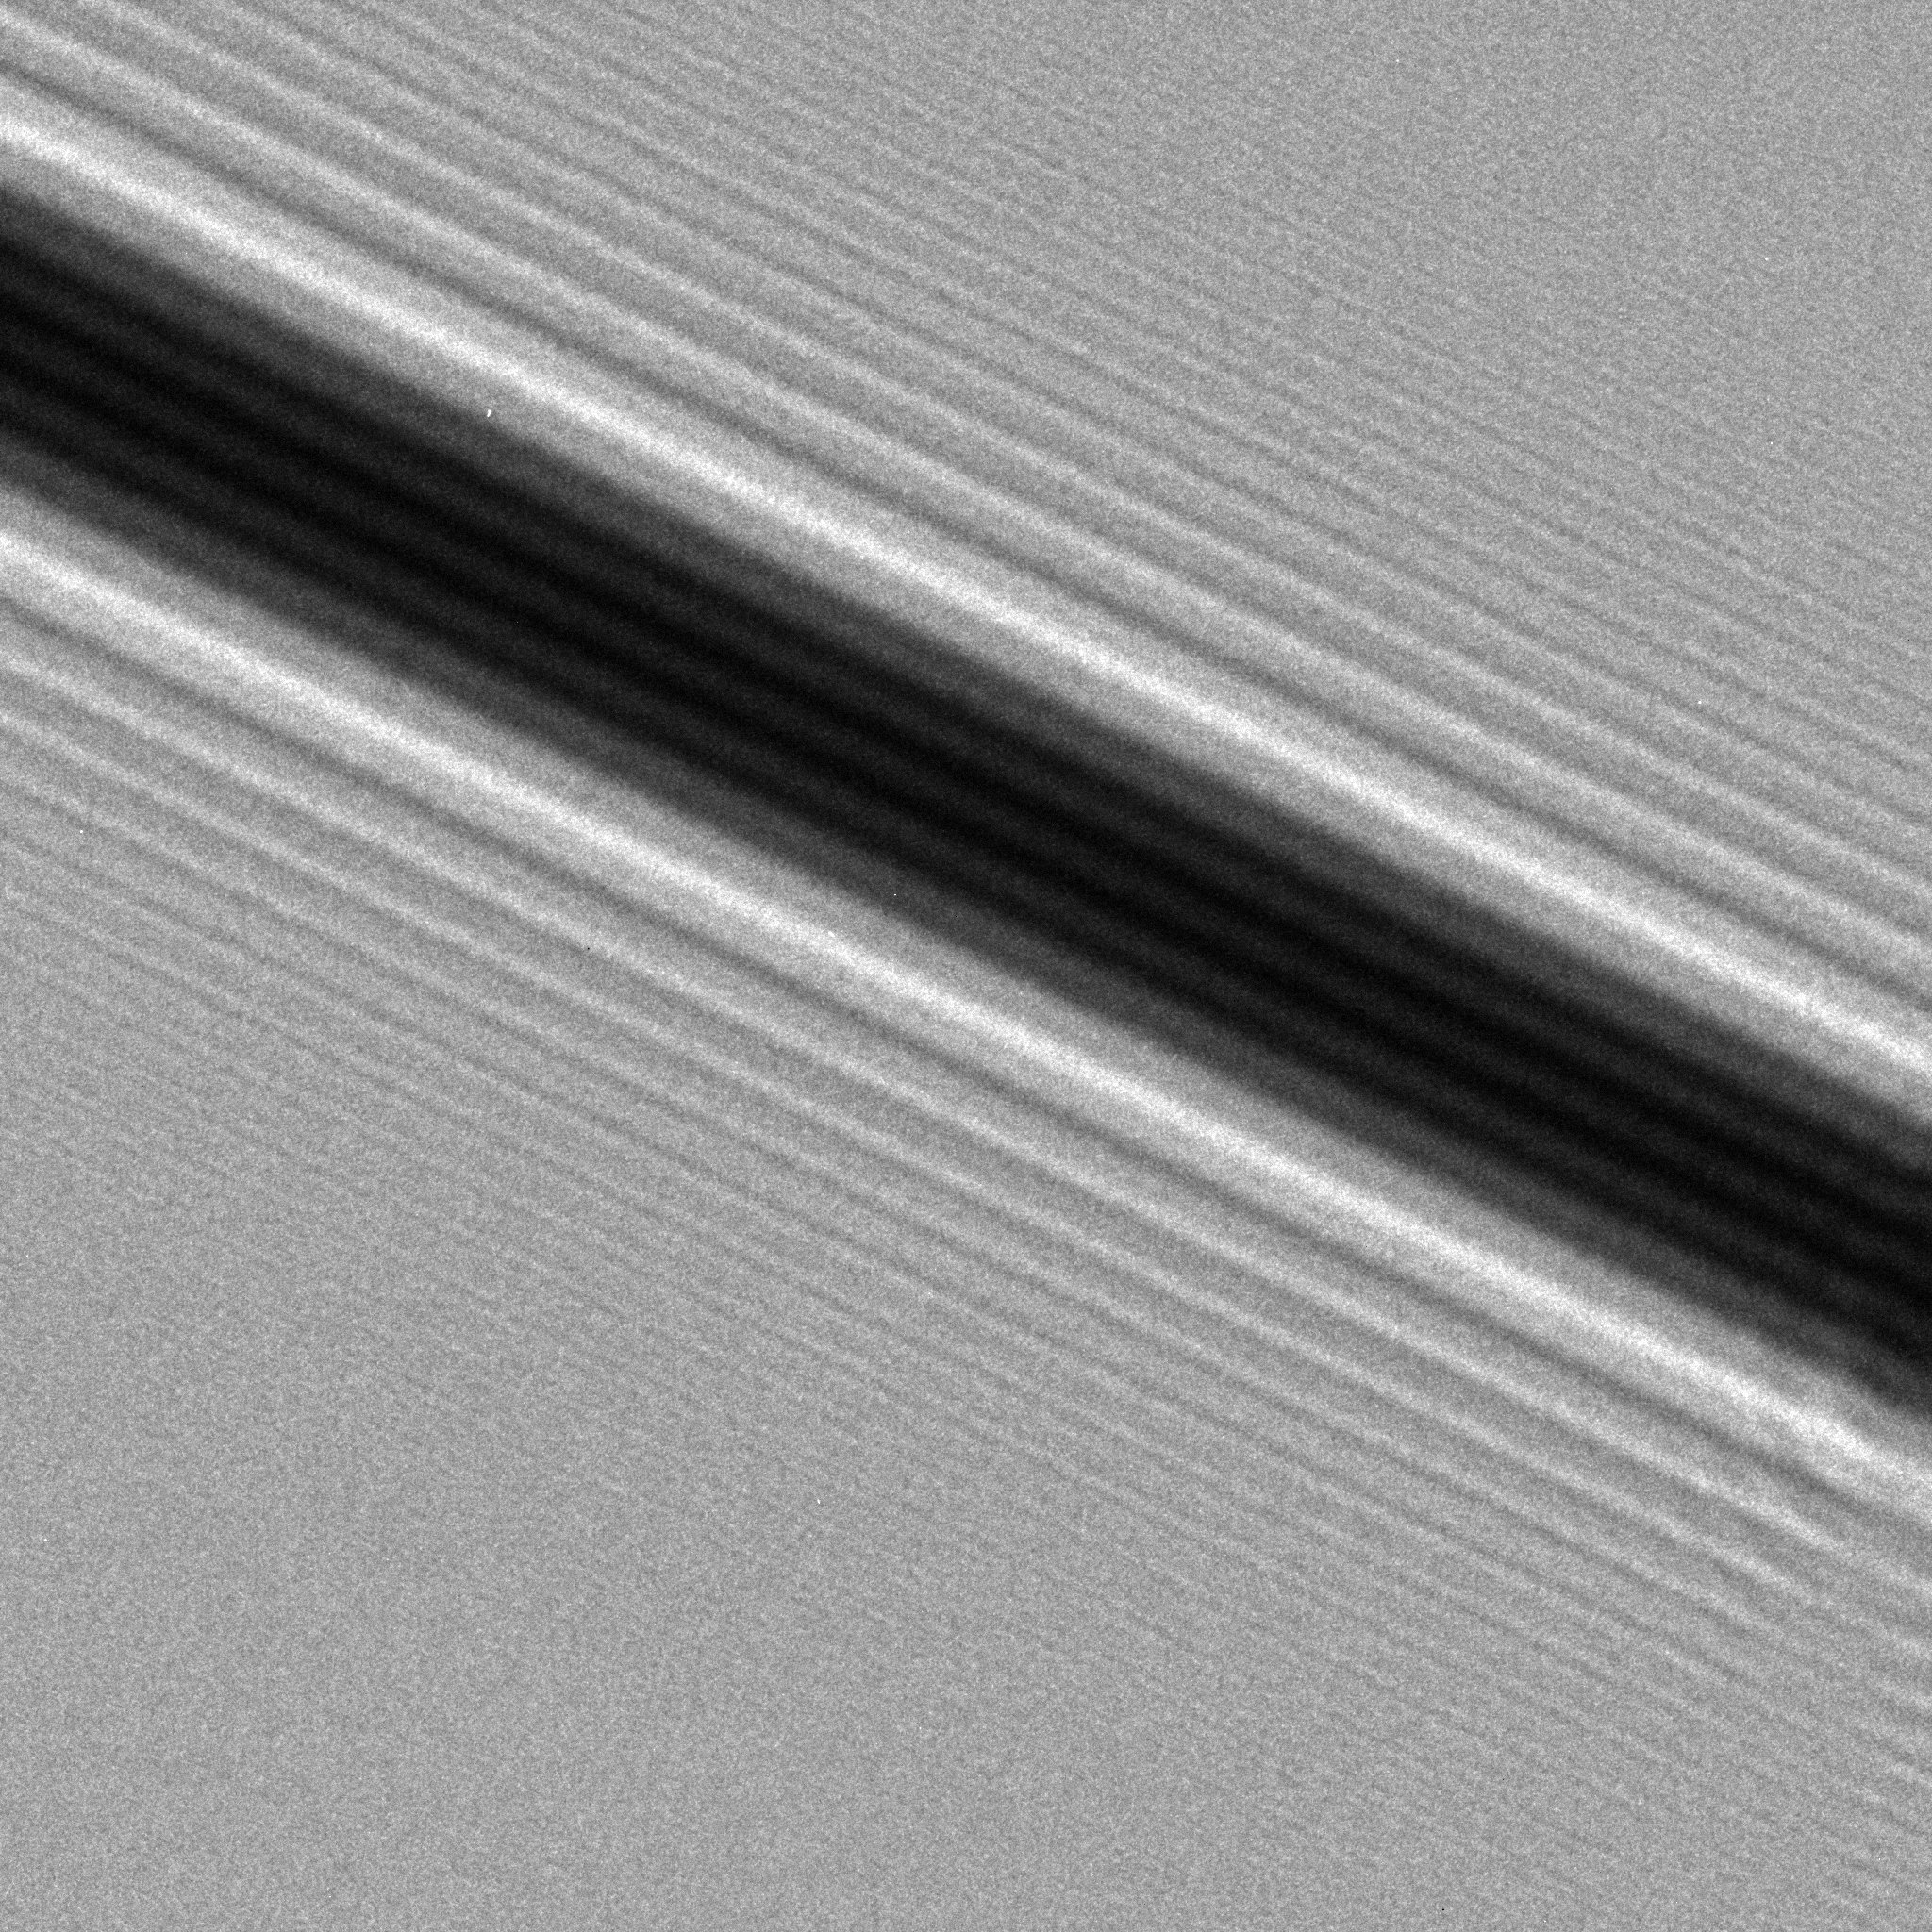
\includegraphics[width=\textwidth]{Holographie/Vakuumhologramm_Rundbeleuchtung/0_02_Vak_Rund.jpg}
         \caption{\(U_F =\) 0,02V}
         \label{002VakRund}
     \end{subfigure}
     \hfill
     \begin{subfigure}[b]{0.49\textwidth}
         \centering
         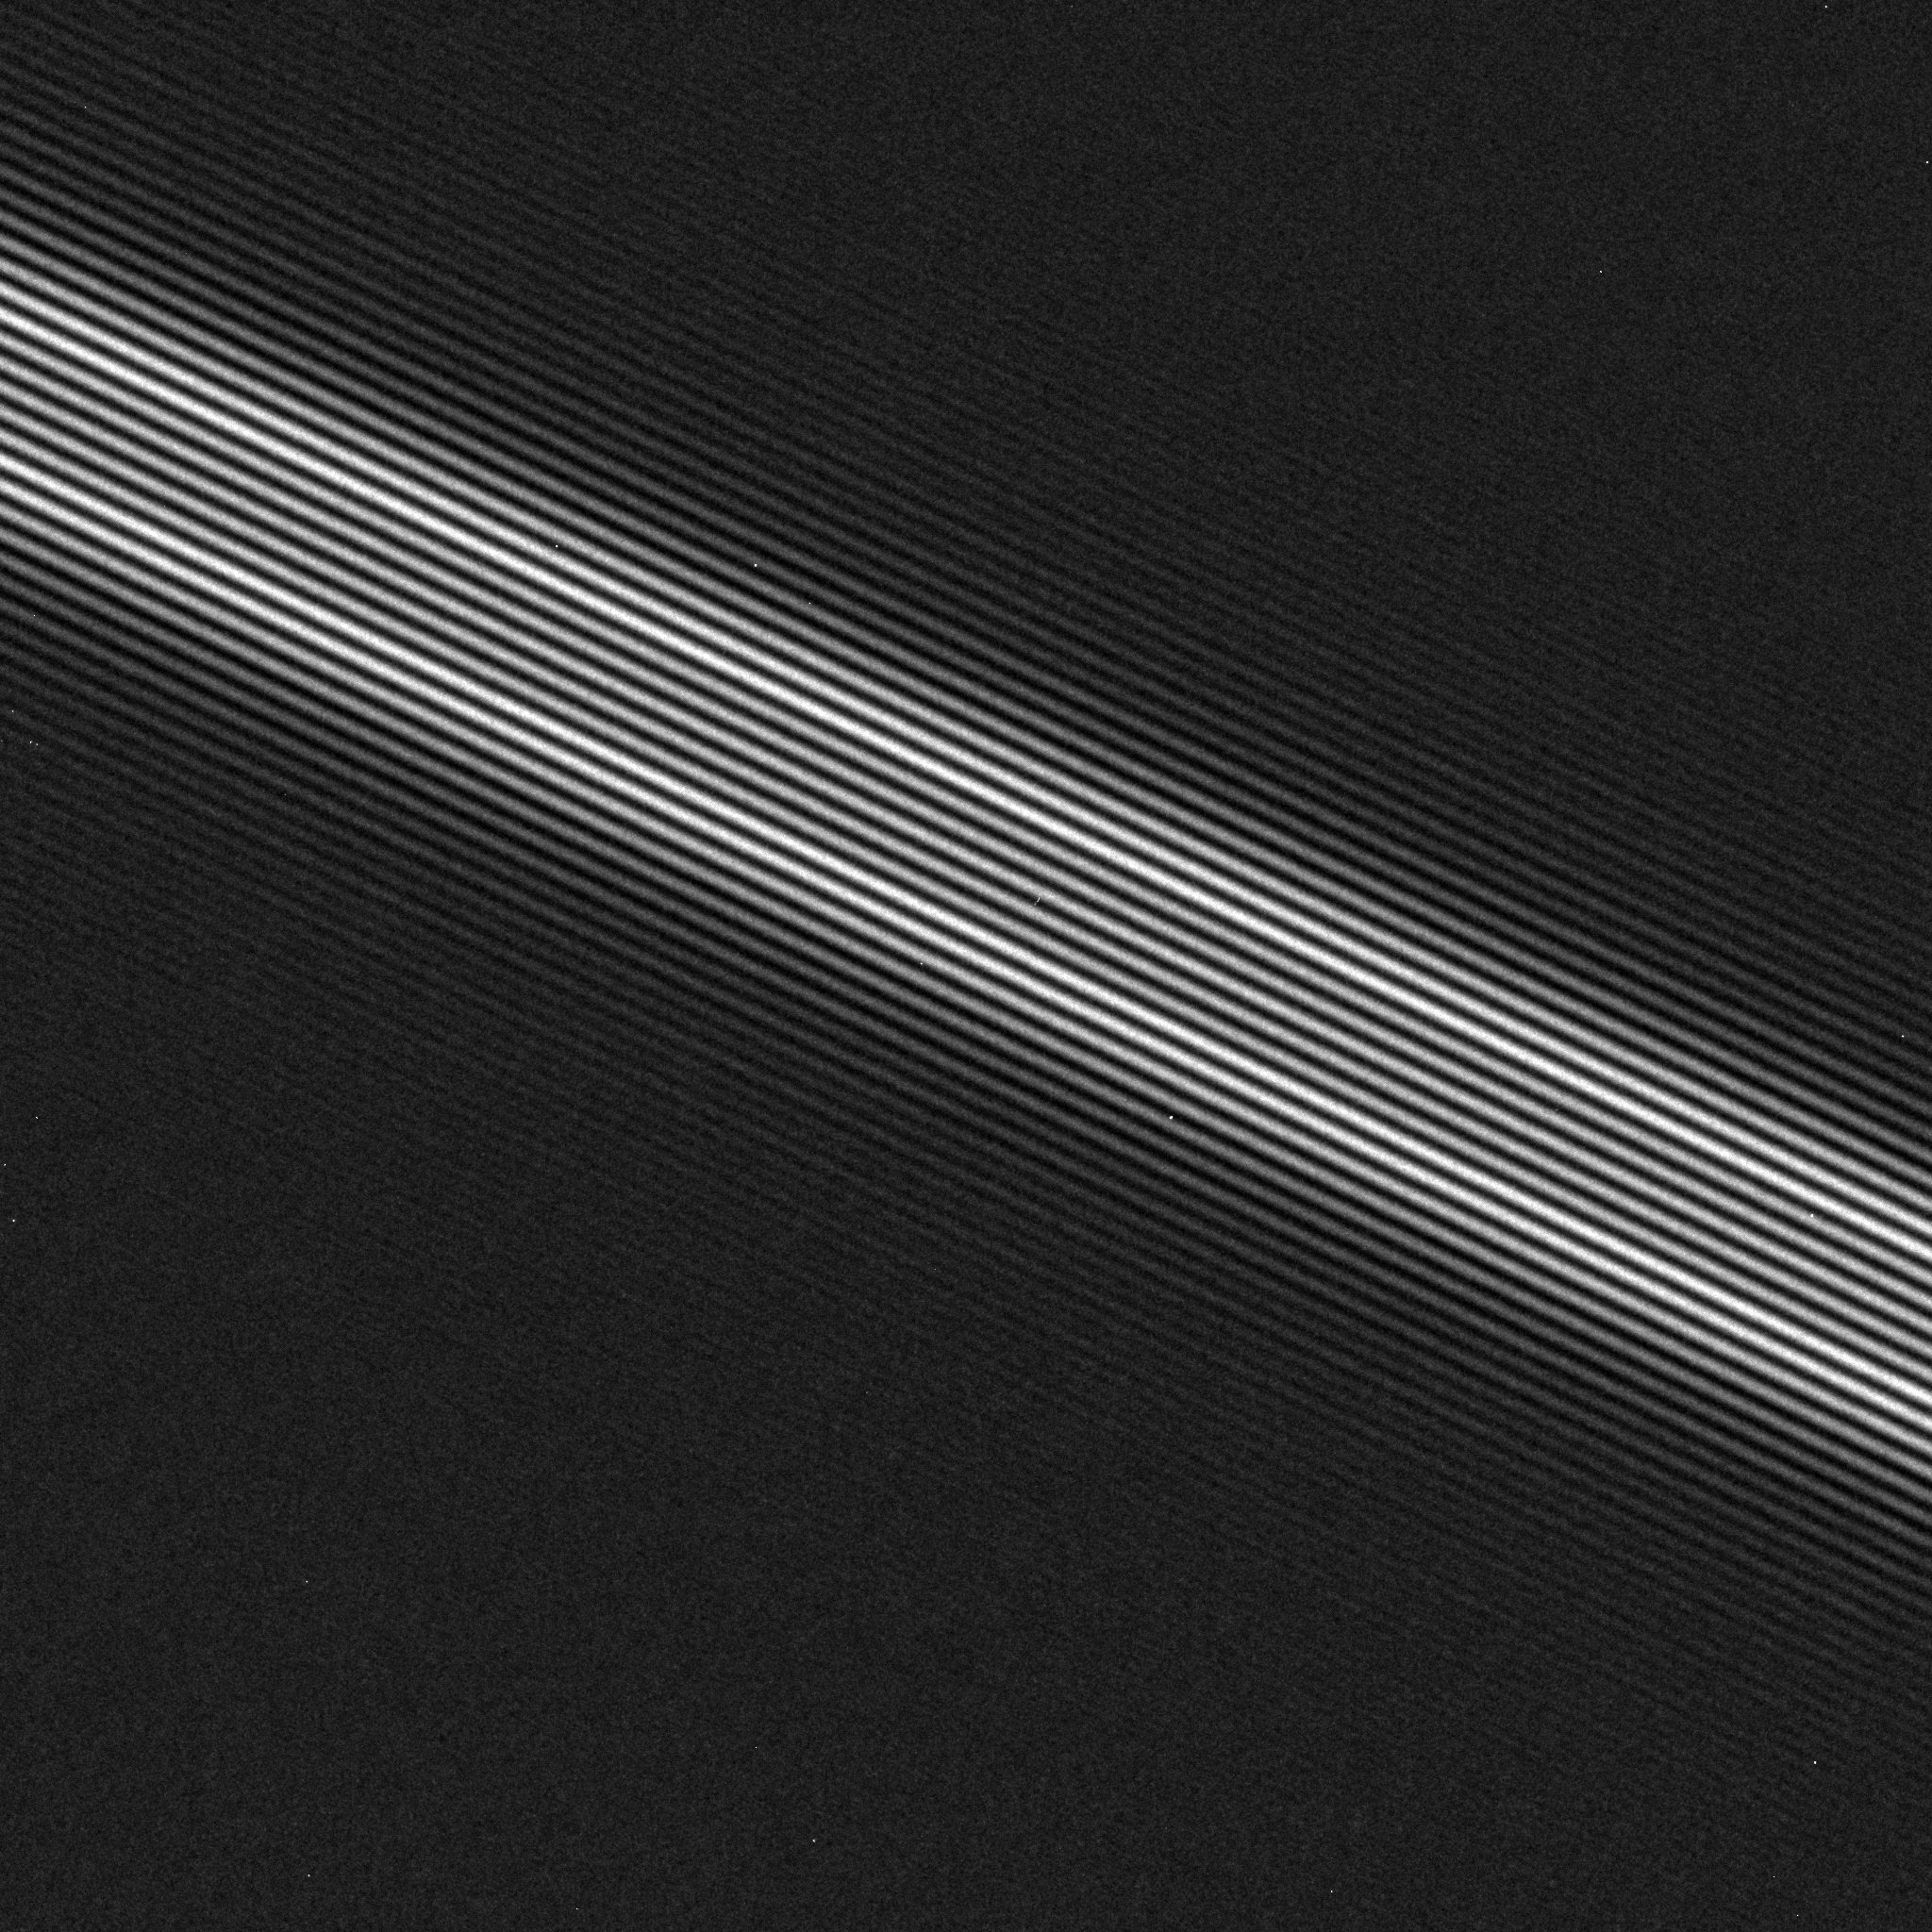
\includegraphics[width=\textwidth]{Holographie/Vakuumhologramm_Rundbeleuchtung/20_4_Vak_Rund.jpg}
         \caption{\(U_F =\) 20,4V}
         \label{204VakRund}
     \end{subfigure}
      
 %\vspace{}

 \centering
     \begin{subfigure}[b]{0.49\textwidth}
         \centering
         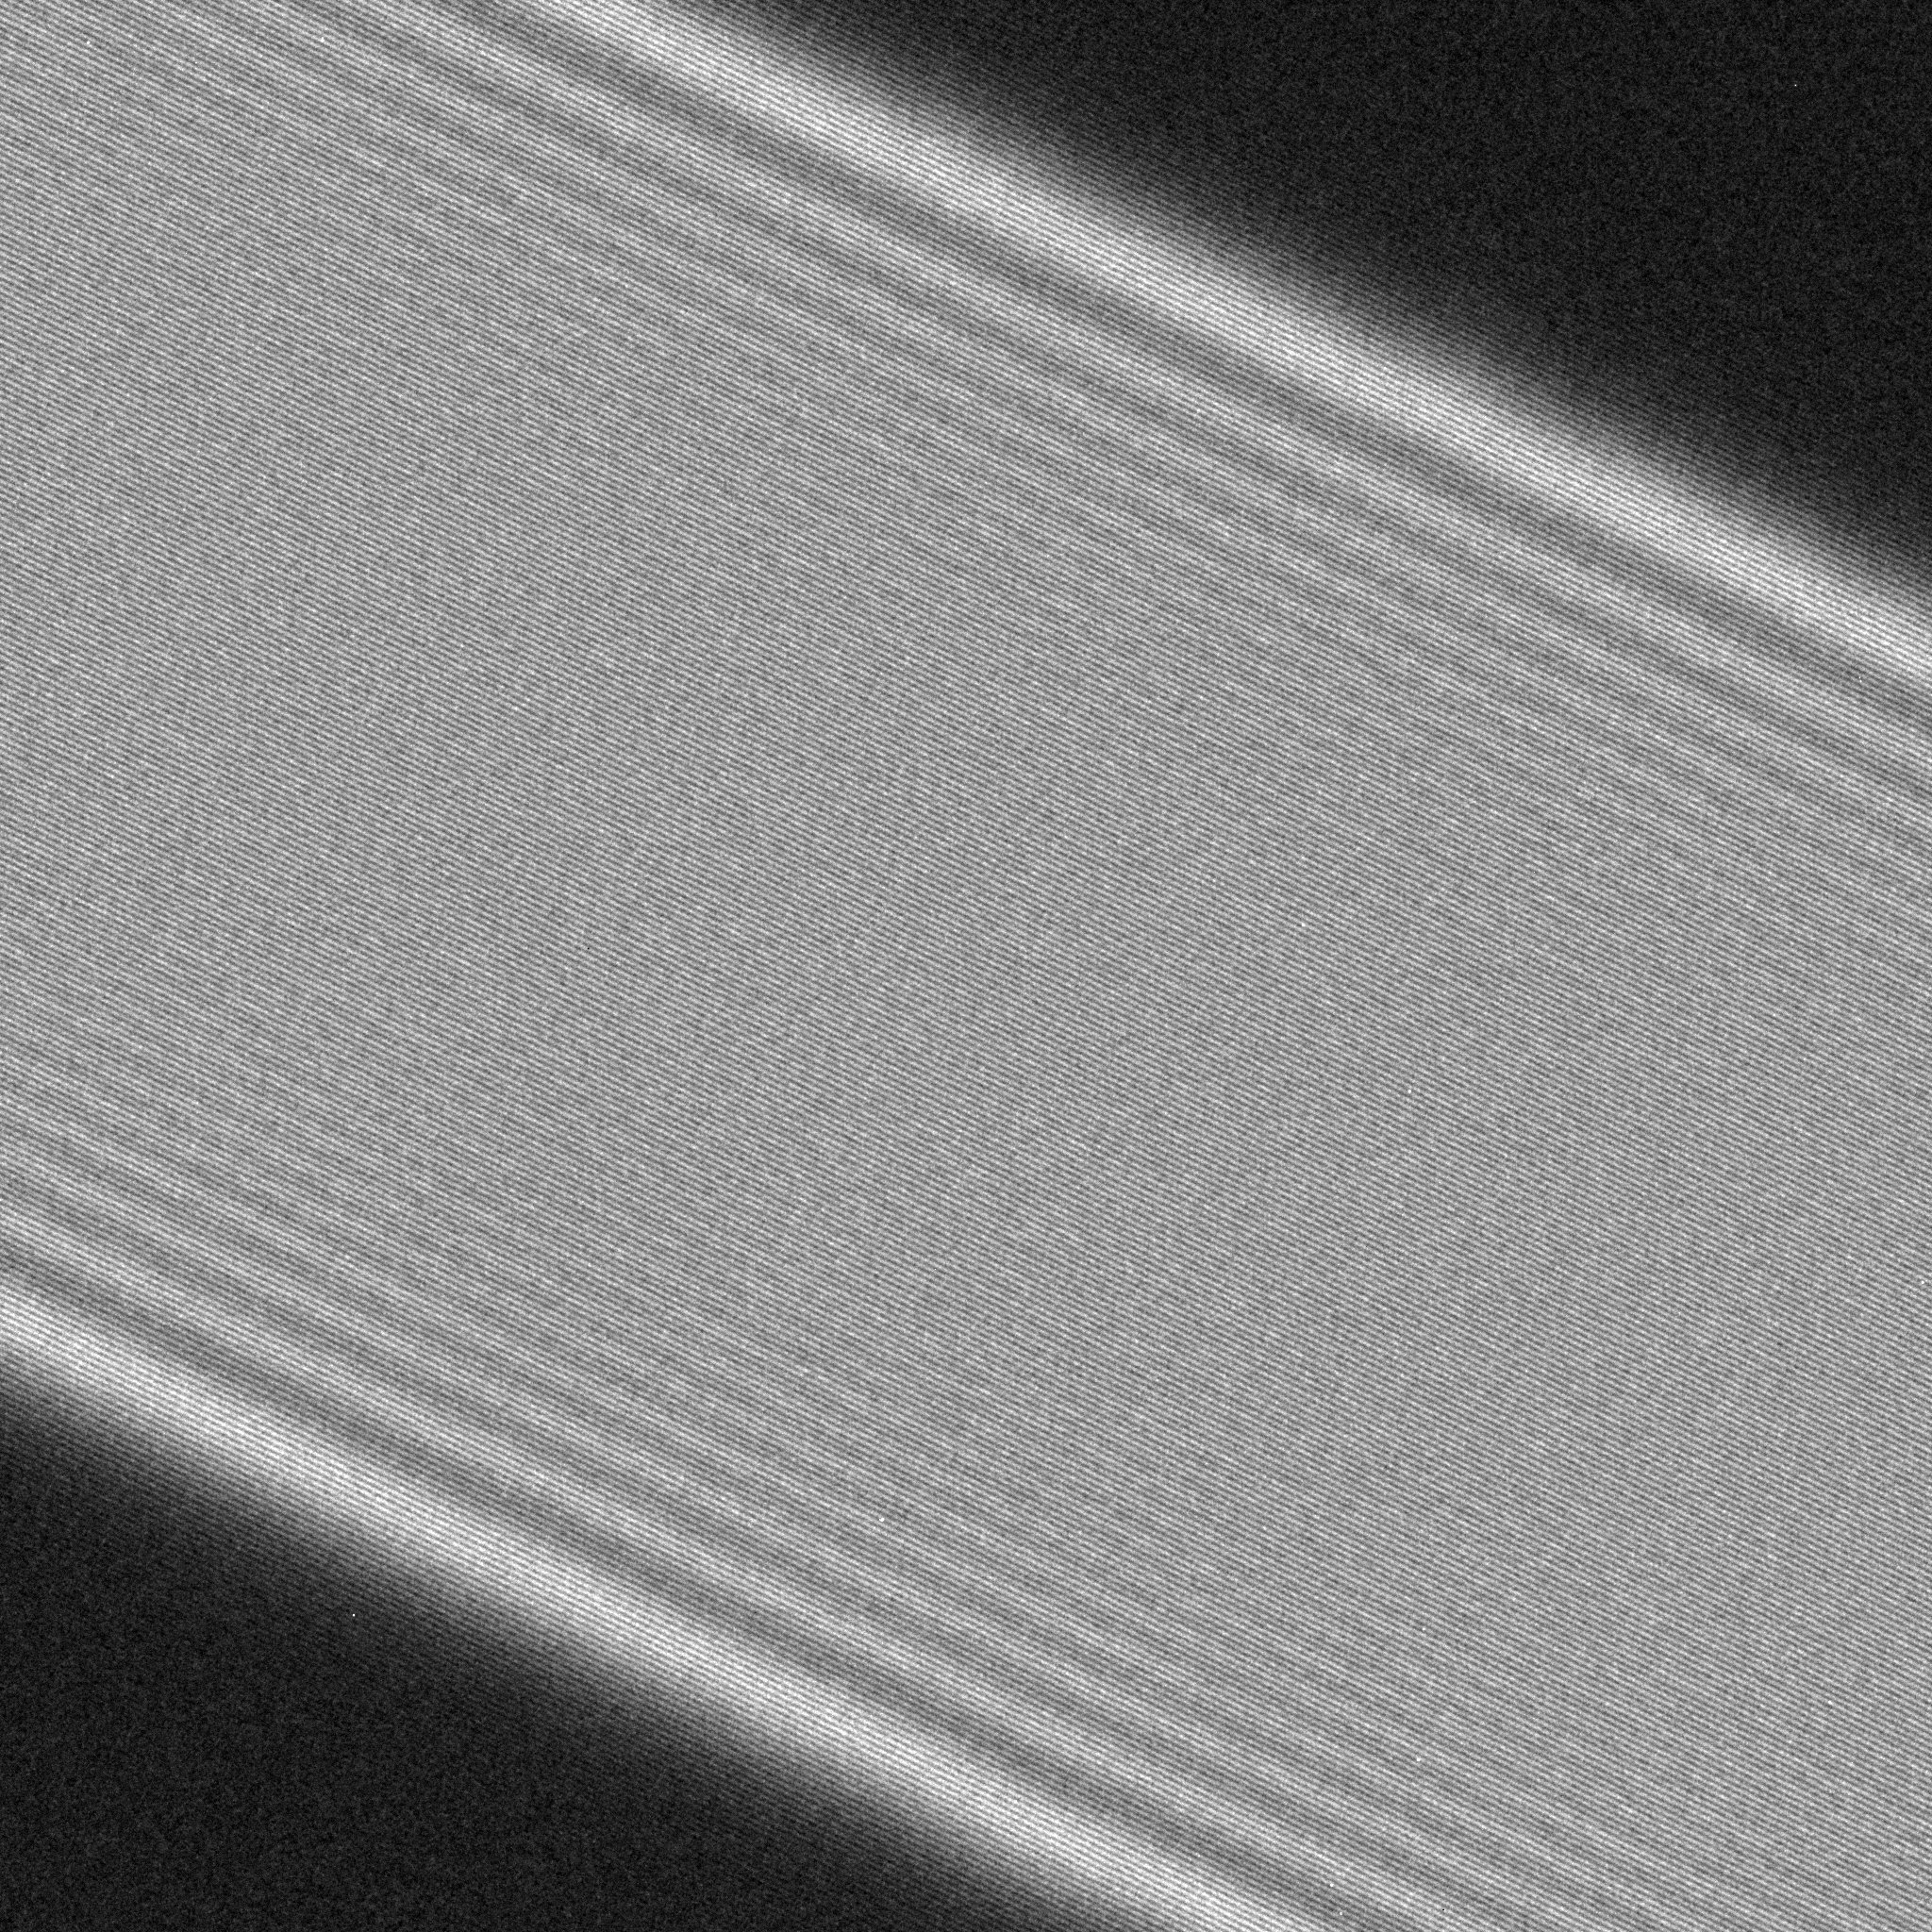
\includegraphics[width=\textwidth]{Holographie/Vakuumhologramm_Rundbeleuchtung/69_8_Vak_Rund.jpg}
         \caption{\(U_F =\) 69,8V}
         \label{698VakRund}
     \end{subfigure}
     \hfill
     \begin{subfigure}[b]{0.49\textwidth}
         \centering
         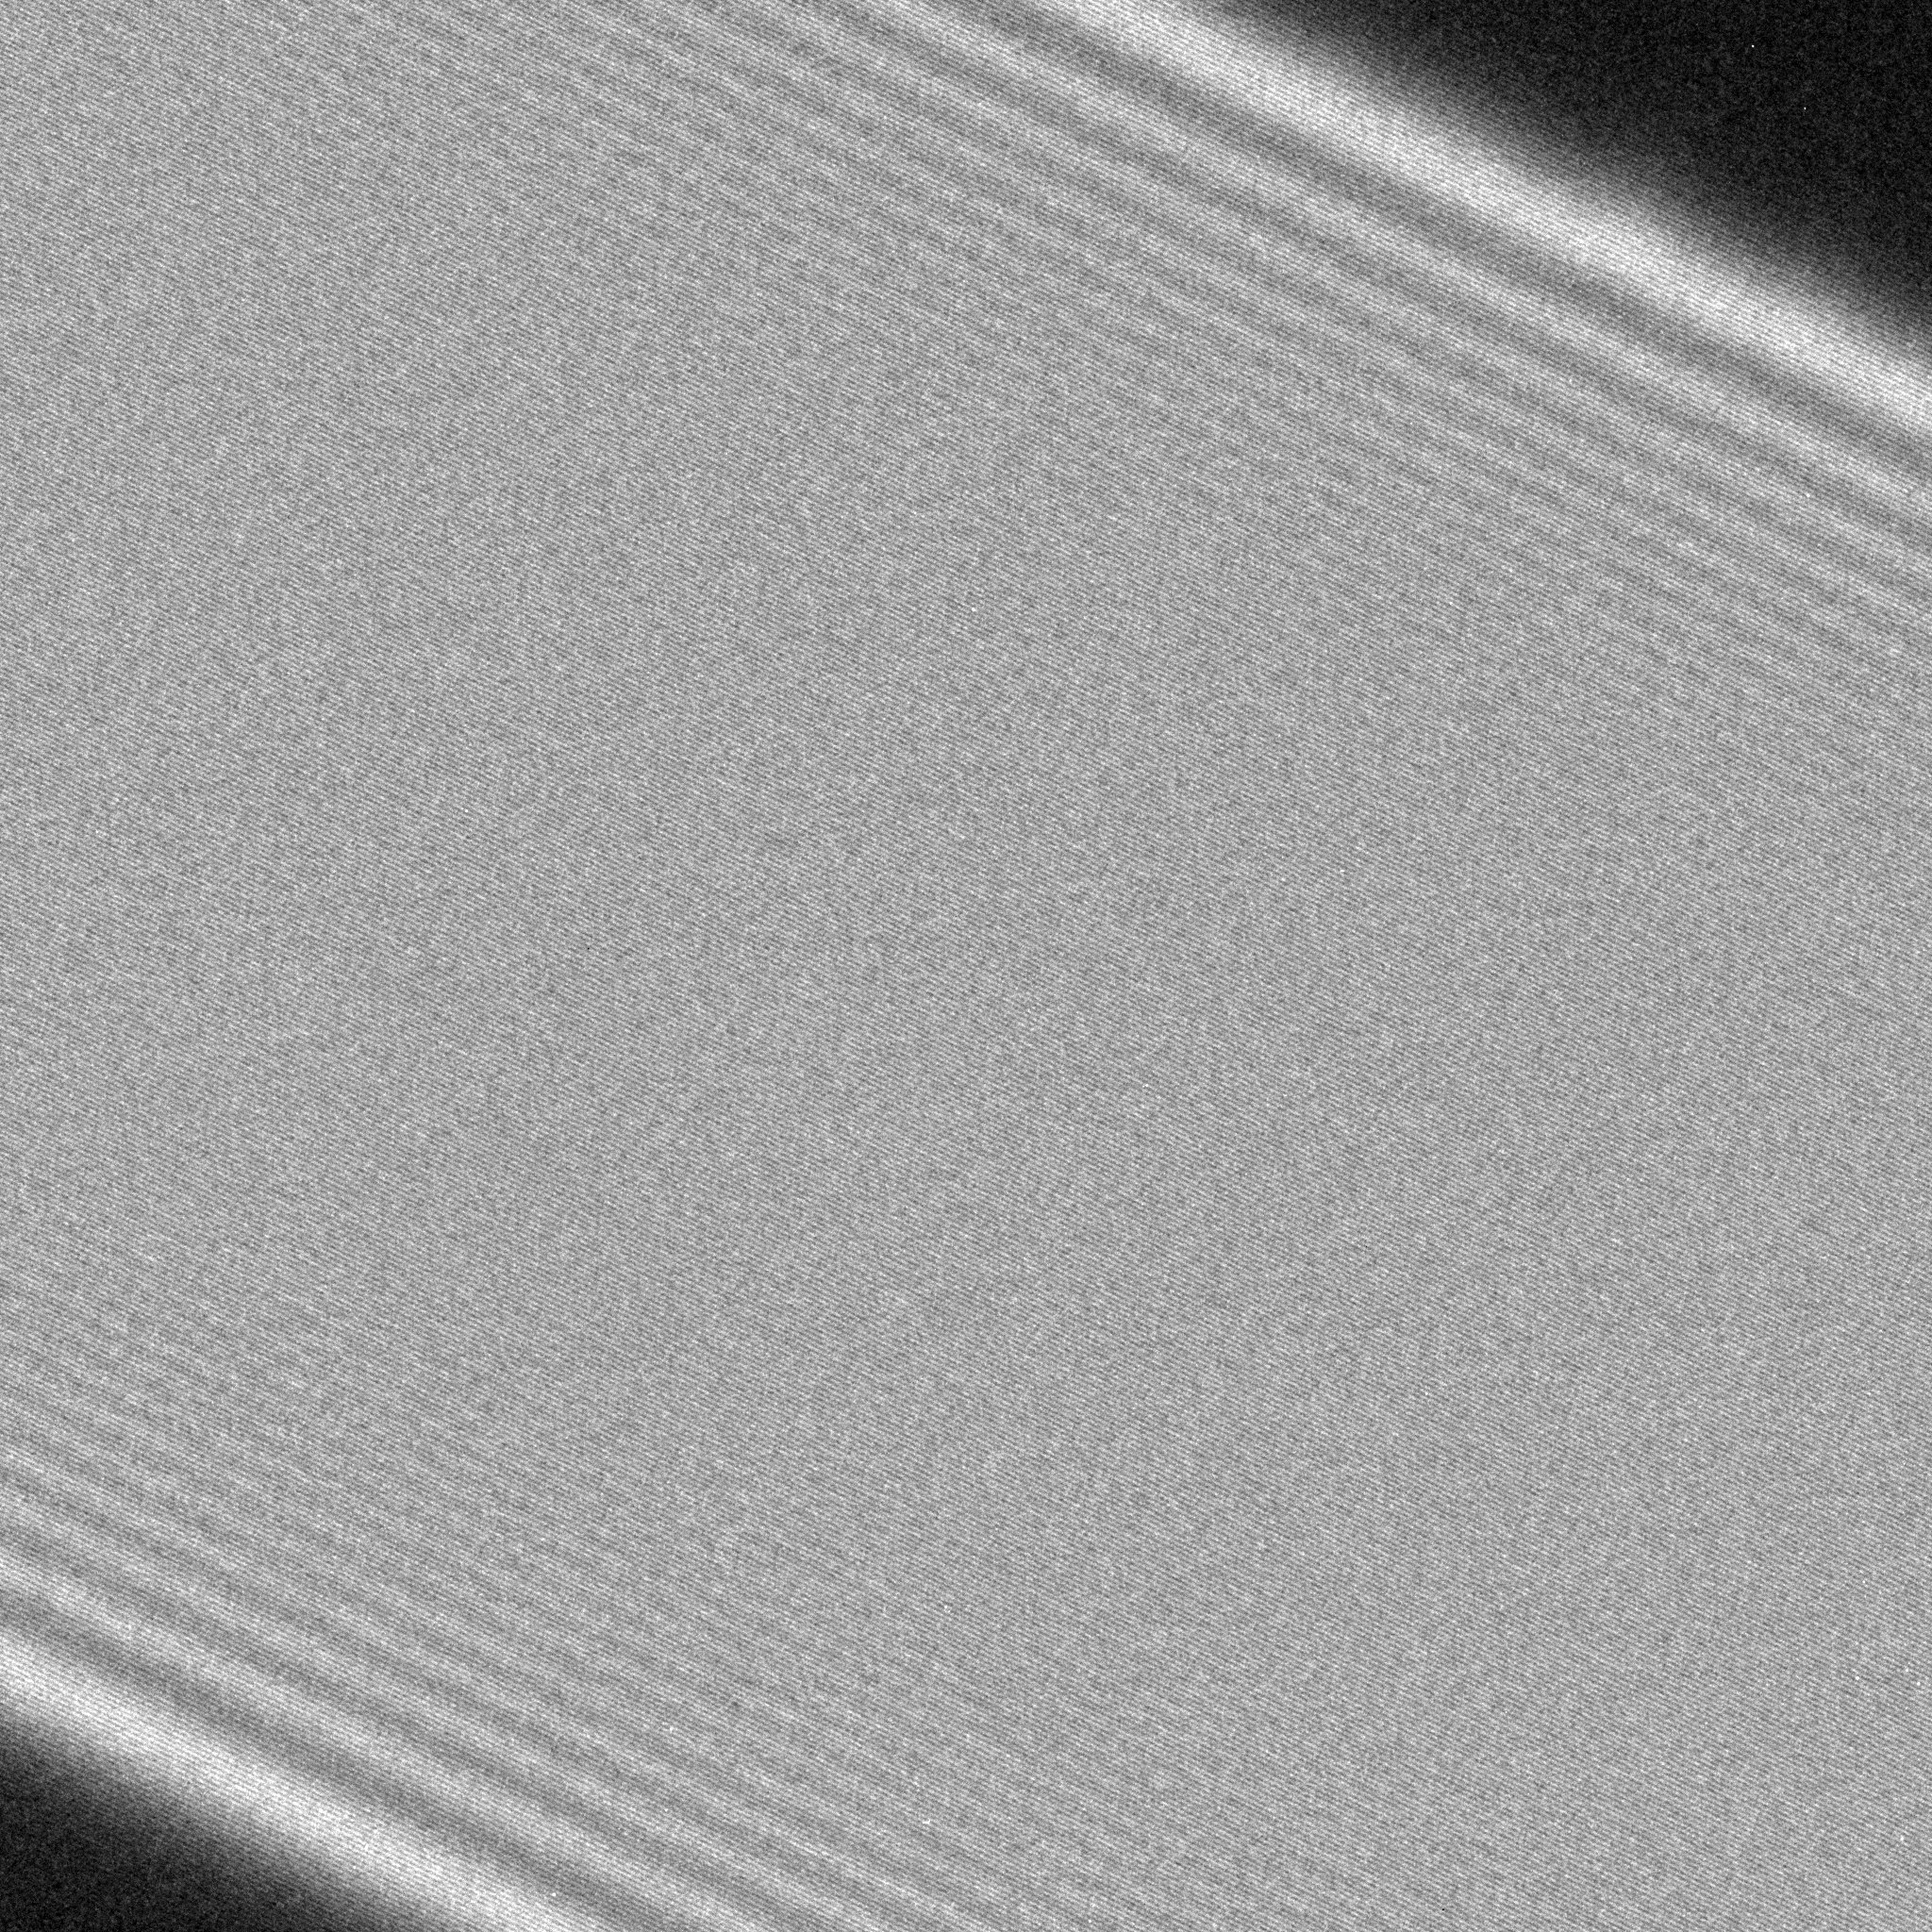
\includegraphics[width=\textwidth]{Holographie/Vakuumhologramm_Rundbeleuchtung/90_4_Vak_Rund.jpg}
         \caption{\(U_F =\) 90,4V}
         \label{904VakRund}
     \end{subfigure}
     \caption{Leerhologramm mit Rundbeleuchtung bei verschiedenen Fadenspannungen}
        \label{VakHolRund}
 
\end{figure}

Bei der Aufnahme ohne eine anliegende Fadenspannung, siehe Bilder \cref{002VakRund}, wird nur leichte Interferenz zwischen den beiden Teilwellen abgebildet, es ist vorallem   Fresnel-Beugung zu sehen. Es ist zusätzlich der durch den Faden verdeckte Elektonenstrahl als Schatten zu erkennen.\\
Bei den Aufnahmen mit einer anliegenden Spannung kann man erkenne das der Interferenzbereich mit zunehmender Spannung größer wird, aber die Interfenz streifen schmaler werden und an Kontrast verlieren. An äußeren Rand des Interferenz Muster kann man weiterhin das Fresnel-Beugung Muster erkennen. \\
Um diese Hologramm Parameter zu quantifizieren wurde ein Skript verwendet, welches in der Lage ist den Streifenkontrast an 5 Punkten der Aufnahme zu messen und angezeigt. Die Interferenzmusterbreite wurde mit der Auswertungssoftware „ImageJ“ gemessen. 

In der Tabelle \cref{VakHolParameter} und den Graphen \cref{VakHolGraph} ist gut zu erkennen wie der Streifenabstand sich mit der Fadenspannung verändert. Die Hologrammbreite nimmt nahezu linear mit der Fadenspannung zu, so wie es durch die Funktion \cref{eq:Hologrammbreite} zu erwarten ist. 

\begin{equation}
\label{eq:Hologrammbreite}
    w_{hol} = 2b \gamma_0 U_F - 2 r_F \frac{a+b}{a}
\end{equation}

\begin{table}[!ht]
    \centering
    \caption{Tabelle der Hologramm Parameter (Steifenabstand, Kontrast und Hologrammbreite) bei unterschiedlichen Biprisma Fadenspannung}
    \begin{tabular}{|l|l|l|l|l|l|l|}
    \hline
        \textbf{Fadenspannung [V]} & \multicolumn{2}{|c|}{\textbf{Kontrast [\%]}} & \multicolumn{2}{|c|}{\textbf{Steifenabstand [Pix]}} & \multicolumn{2}{|c|}{\textbf{Breite [Pix]}} \\ \hline
        \textbf{Beleuchtung:} & Rund & Eliptisch & Rund & Eliptisch & Rund & Eliptisch \\ \hline
        \textbf{0} & 0.62 & 0.92 & 17.7 & 18.25 & 0 & 0 \\ 
        \textbf{10} & 0.35 & 4.5 & 9.17 & 18.29 & 295.945 & 275.476 \\ 
        \textbf{20} & 0.35 & 40.04 & 18.24 & 15.7 & 334.632 & 399.259 \\ 
        \textbf{30} & 37.67 & 31.77 & 15.46 & 11.91 & 419.34 & 517.229 \\ 
        \textbf{40} & 29.2 & 31.36 & 12.08 & 11.76 & 525.395 & 541.194 \\ 
        \textbf{50} & 22.18 & 25.16 & 9.53 & 9.69 & 643.836 & 654.702 \\ 
        \textbf{60} & 17.19 & 20.26 & 8.12 & 7.95 & 796.13 & 816.493 \\ 
        \textbf{70} & 13.62 & 16.45 & 6.99 & 6.96 & 914.647 & 931.022 \\ 
        \textbf{80} & 10.46 & 12.34 & 6.08 & 6.04 & 1104.862 & 1098.322 \\ 
        \textbf{90} & 7.65 & 10.14 & 5.41 & 5.42 & 1261.25 & 1228.854 \\ \hline
    \end{tabular}
    \label{VakHolParameter}
\end{table}

\begin{figure}
     \centering
     \begin{subfigure}[b]{0.3\textwidth}
         \centering
         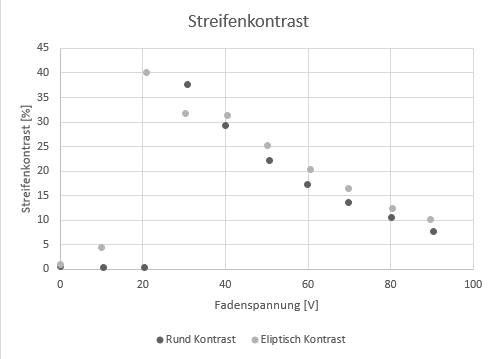
\includegraphics[width=\textwidth]{Holographie/Vakuumhologramm_Rundbeleuchtung/Kontrast.png}
         \caption{Kontrast}
         \label{LeerHolKontrast}
     \end{subfigure}
     \hfill
     \begin{subfigure}[b]{0.3\textwidth}
         \centering
         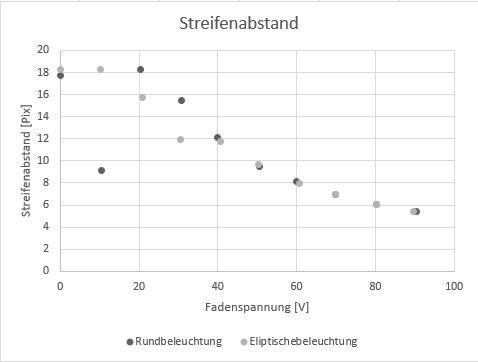
\includegraphics[width=\textwidth]{Holographie/Vakuumhologramm_Rundbeleuchtung/Streifenabstand.png}
         \caption{Streifenabstand}
         \label{LeerHolStreifenabstand}
     \end{subfigure}
     \hfill
     \begin{subfigure}[b]{0.3\textwidth}
         \centering
         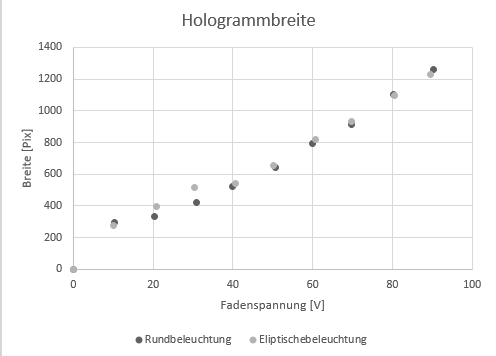
\includegraphics[width=\textwidth]{Holographie/Vakuumhologramm_Rundbeleuchtung/Hologrammbreite.png}
         \caption{Hologrammbreite}
         \label{StreifenabstandBreite}
     \end{subfigure}
        \caption{Plots der Steifenabstand, Kontrast und Hologrammbreite in Leerhologrammen bei Rund und Elliptischer Beleuchtung für verschiedene Fadenspannungen}
        \label{VakHolGraph}
\end{figure}

Der streifenabstand hingegen wird durch Formel \cref{Streifenabstand} beschriebenen und gibt eine inversproportionale Abhängigkeit von der Fadenspannung an. Diese kann auch beobachtet werden, jedoch nicht bei geringeren Fadenspannung

\begin{equation}
\label{Streifenabstand}
    s_{hol} = \frac{1}{q_c} = \frac{a+b}{2 k a \gamma_0 U_F}
\end{equation}

Der Kontrast hat seinen Maxima bei einer Fadenspannung von ca. 30V mit einer runden Beleuchtung und 20V bei der elliptischen Beleuchtung. Auf die Kontrast Abhängigkeit von Fadenspannung und Beleuchtung wird oben weiter eingegangen.\\
Um den Streifenkontrast des Hologramms zu erhöhen, wurde nun die Beleuchtung von der runden Beleuchtung auf eine elliptische Beleuchtung umgestellt. Dafür wurde die Stigmator Einstellungen so angepasst das der Elliptisch geformte Strahl senkrecht zur Biprisma Faden stand. Durch den stärker zusammengezogenen Strahl und die dadurch entstandenen höheren gemessenen Elektronen Zahl auf dem CCD-Kamera, musste die Beleuchtungszeit auf der Kamera auf 2 Sekunden verkürzt werden, um Überbelichtung zu vermeiden.

Anschließend wurde die Messreihe mit verschiedenen Fadenspannung analog zur rund Beleuchtung für eine Elliptische Beleuchtung widerholt. Siehe Abbildung \cref{VakHolEllip} Im Vergleich zur runden Beleuchtung ist jetzt ein sehr viel besserer Streifenkontrast zu erkennen. 
In der \cref{VakHolParameter} sind sie Ergebnisse zusammengefast, um Graphen \cref{VakHolGraph} dargestellt.

\begin{figure}[H]
     \centering
     \begin{subfigure}[b]{0.49\textwidth}
         \centering
         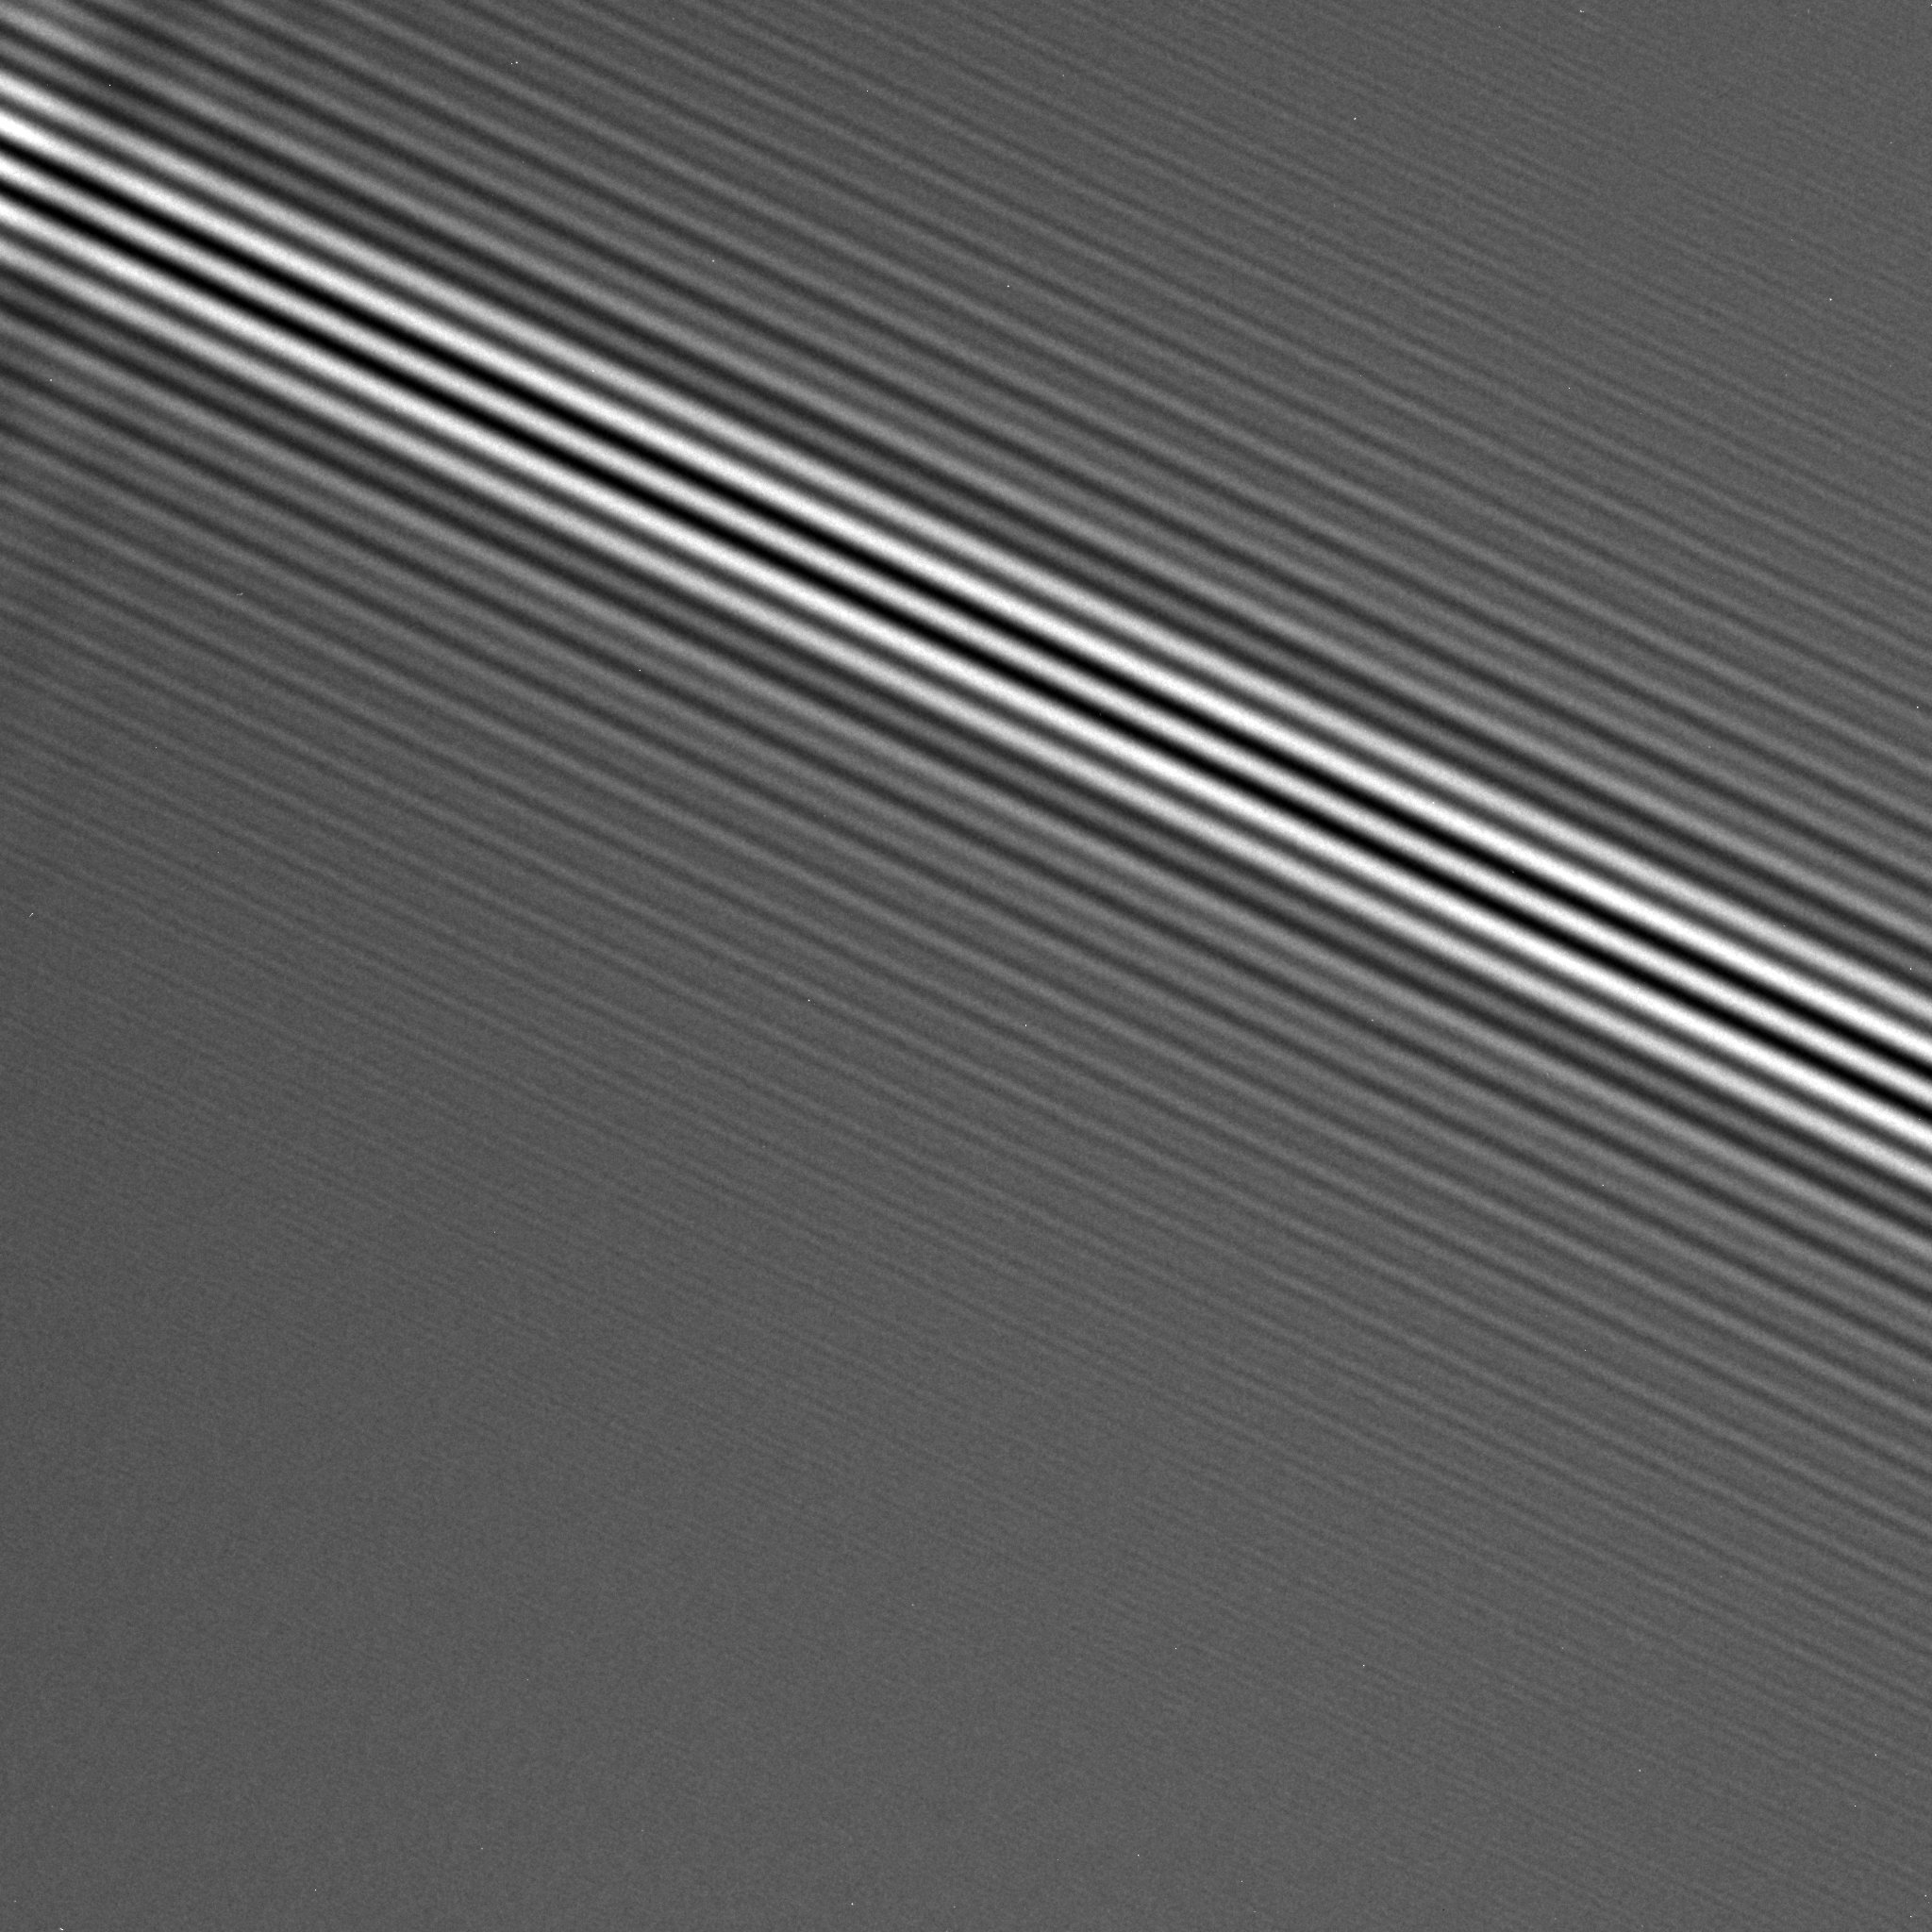
\includegraphics[width=\textwidth]{Holographie/Vakuumhologramm_Elliptischebeleuchtung/0_02_Vak_Ellip.jpg}
         \caption{\(U_F =\) 0,02V}
         \label{002VakEllip}
     \end{subfigure}
     \hfill
     \begin{subfigure}[b]{0.49\textwidth}
         \centering
         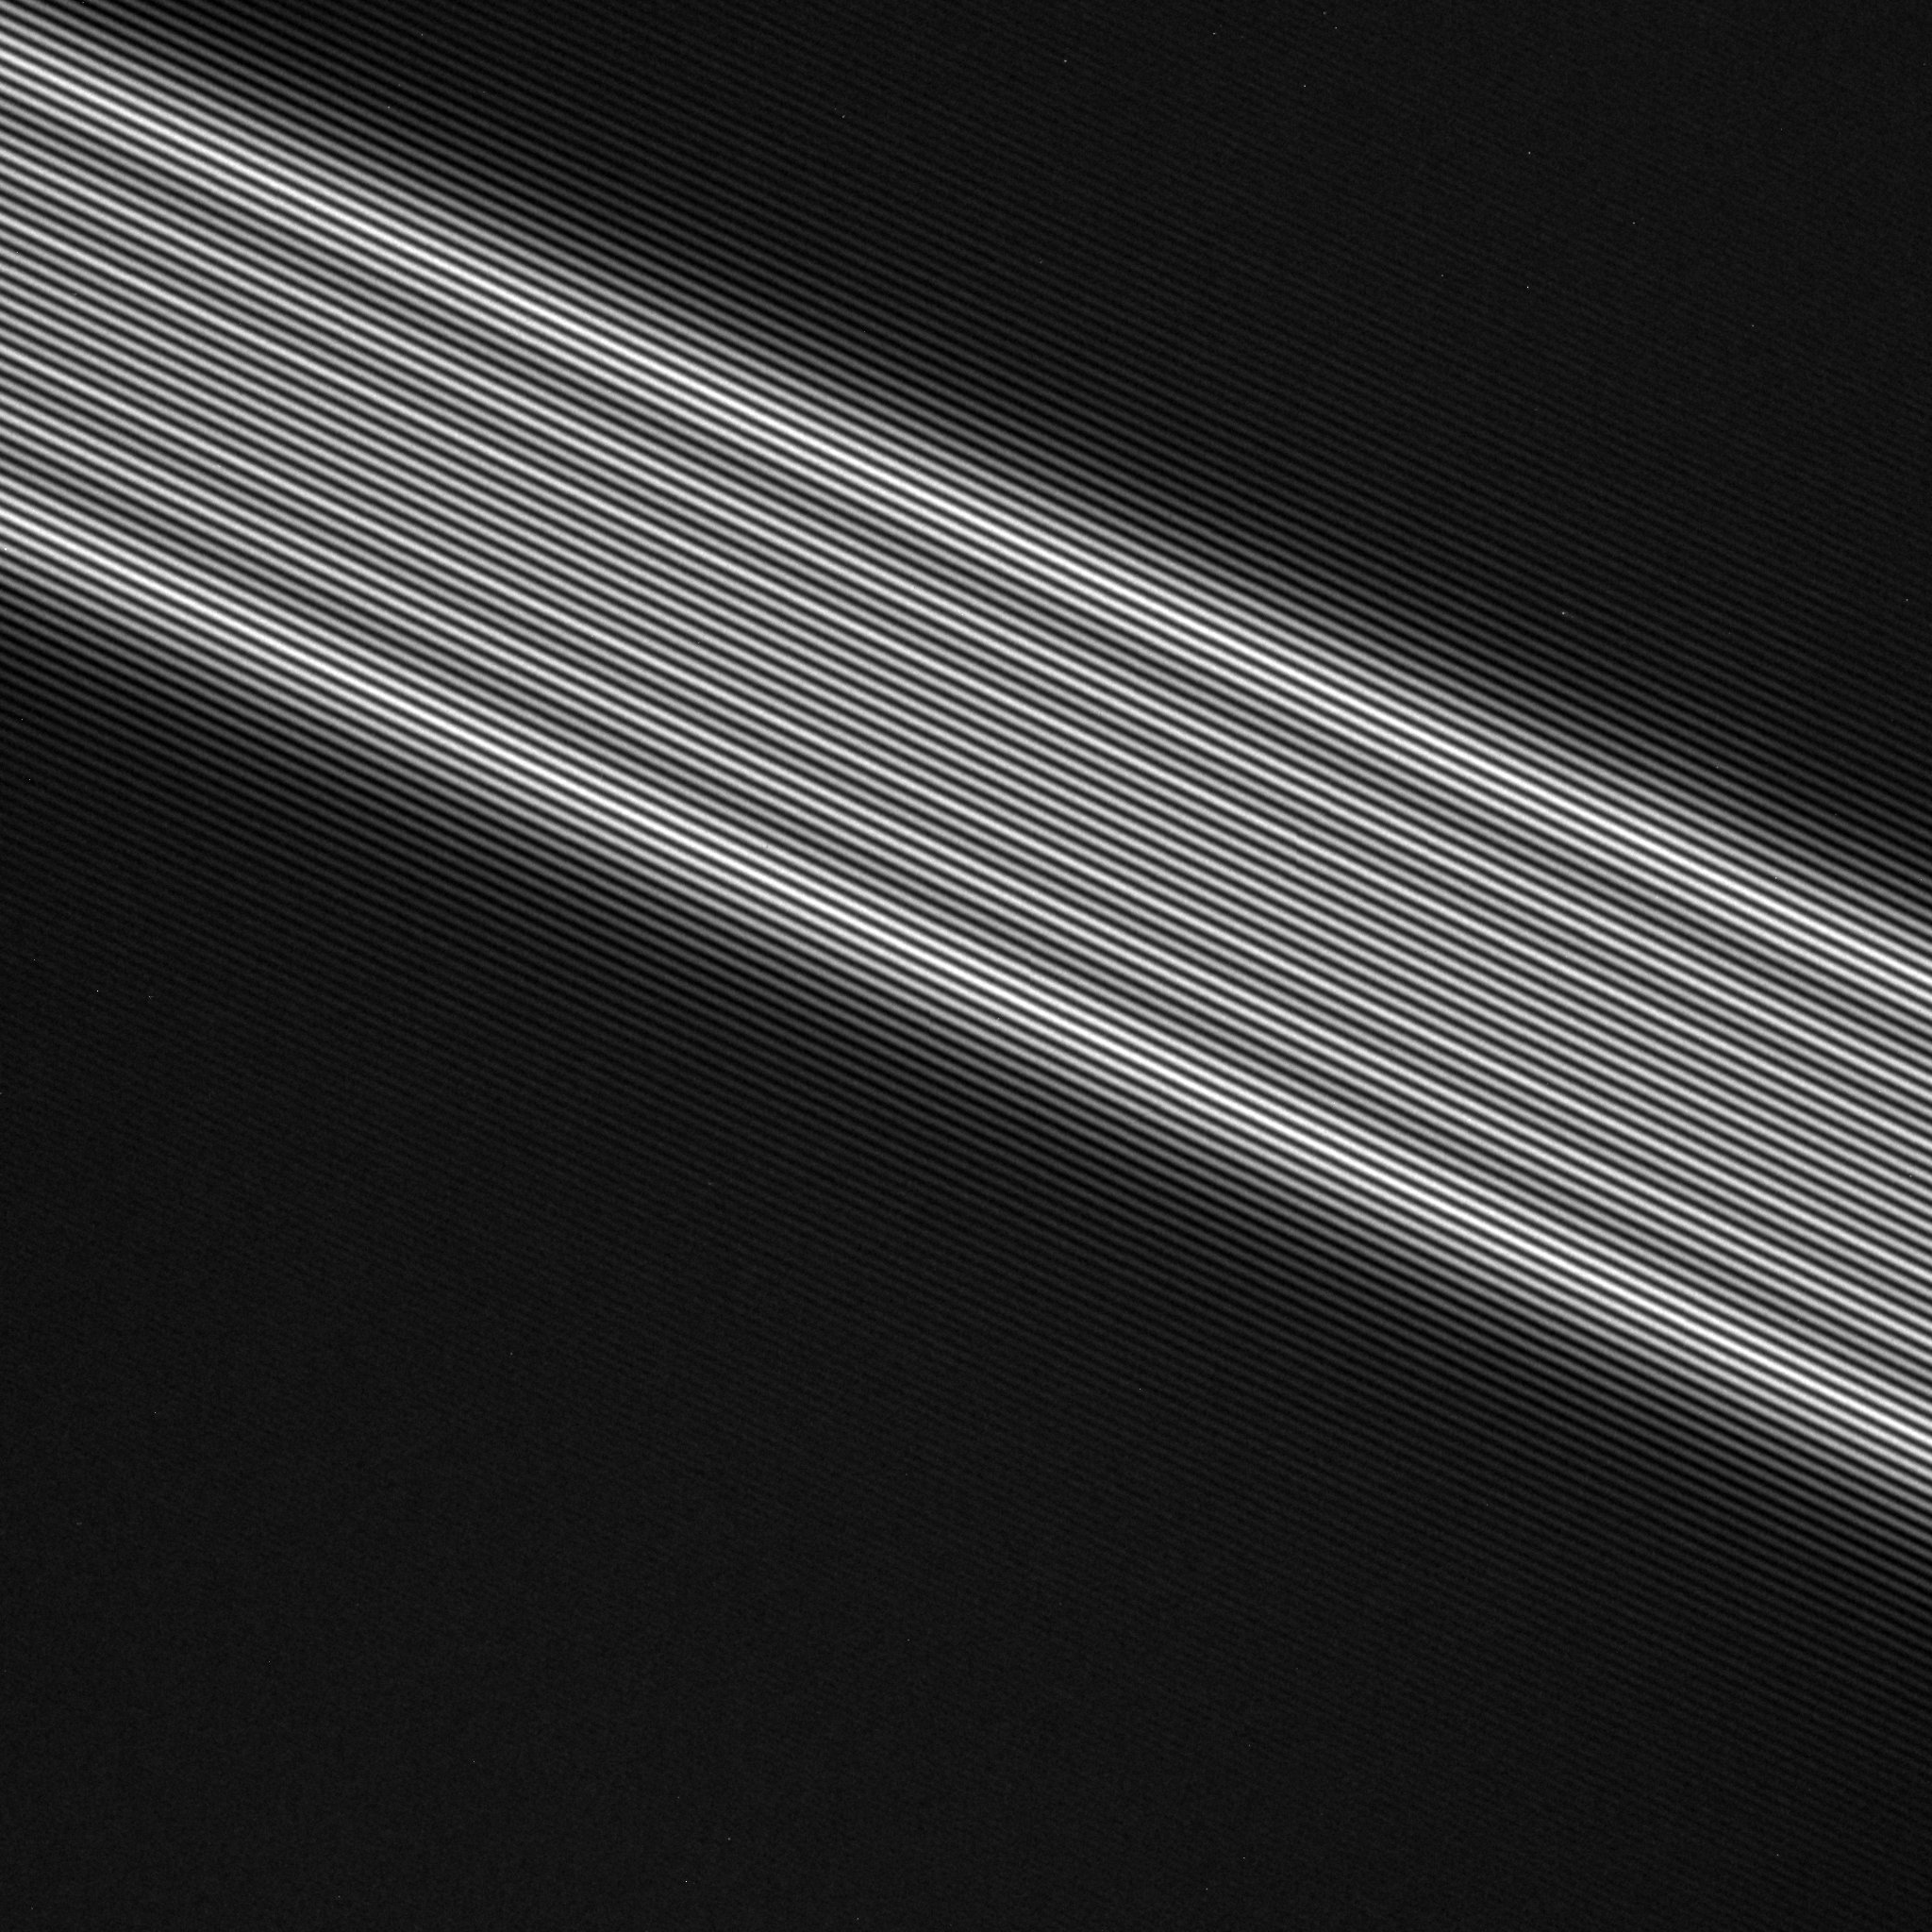
\includegraphics[width=\textwidth]{Holographie/Vakuumhologramm_Elliptischebeleuchtung/20_8_Vak_Ellip.jpg}
         \caption{\(U_F =\) 20,8V}
         \label{208VakEllip}
     \end{subfigure}
      
 %\vspace{}

 \centering
     \begin{subfigure}[b]{0.49\textwidth}
         \centering
         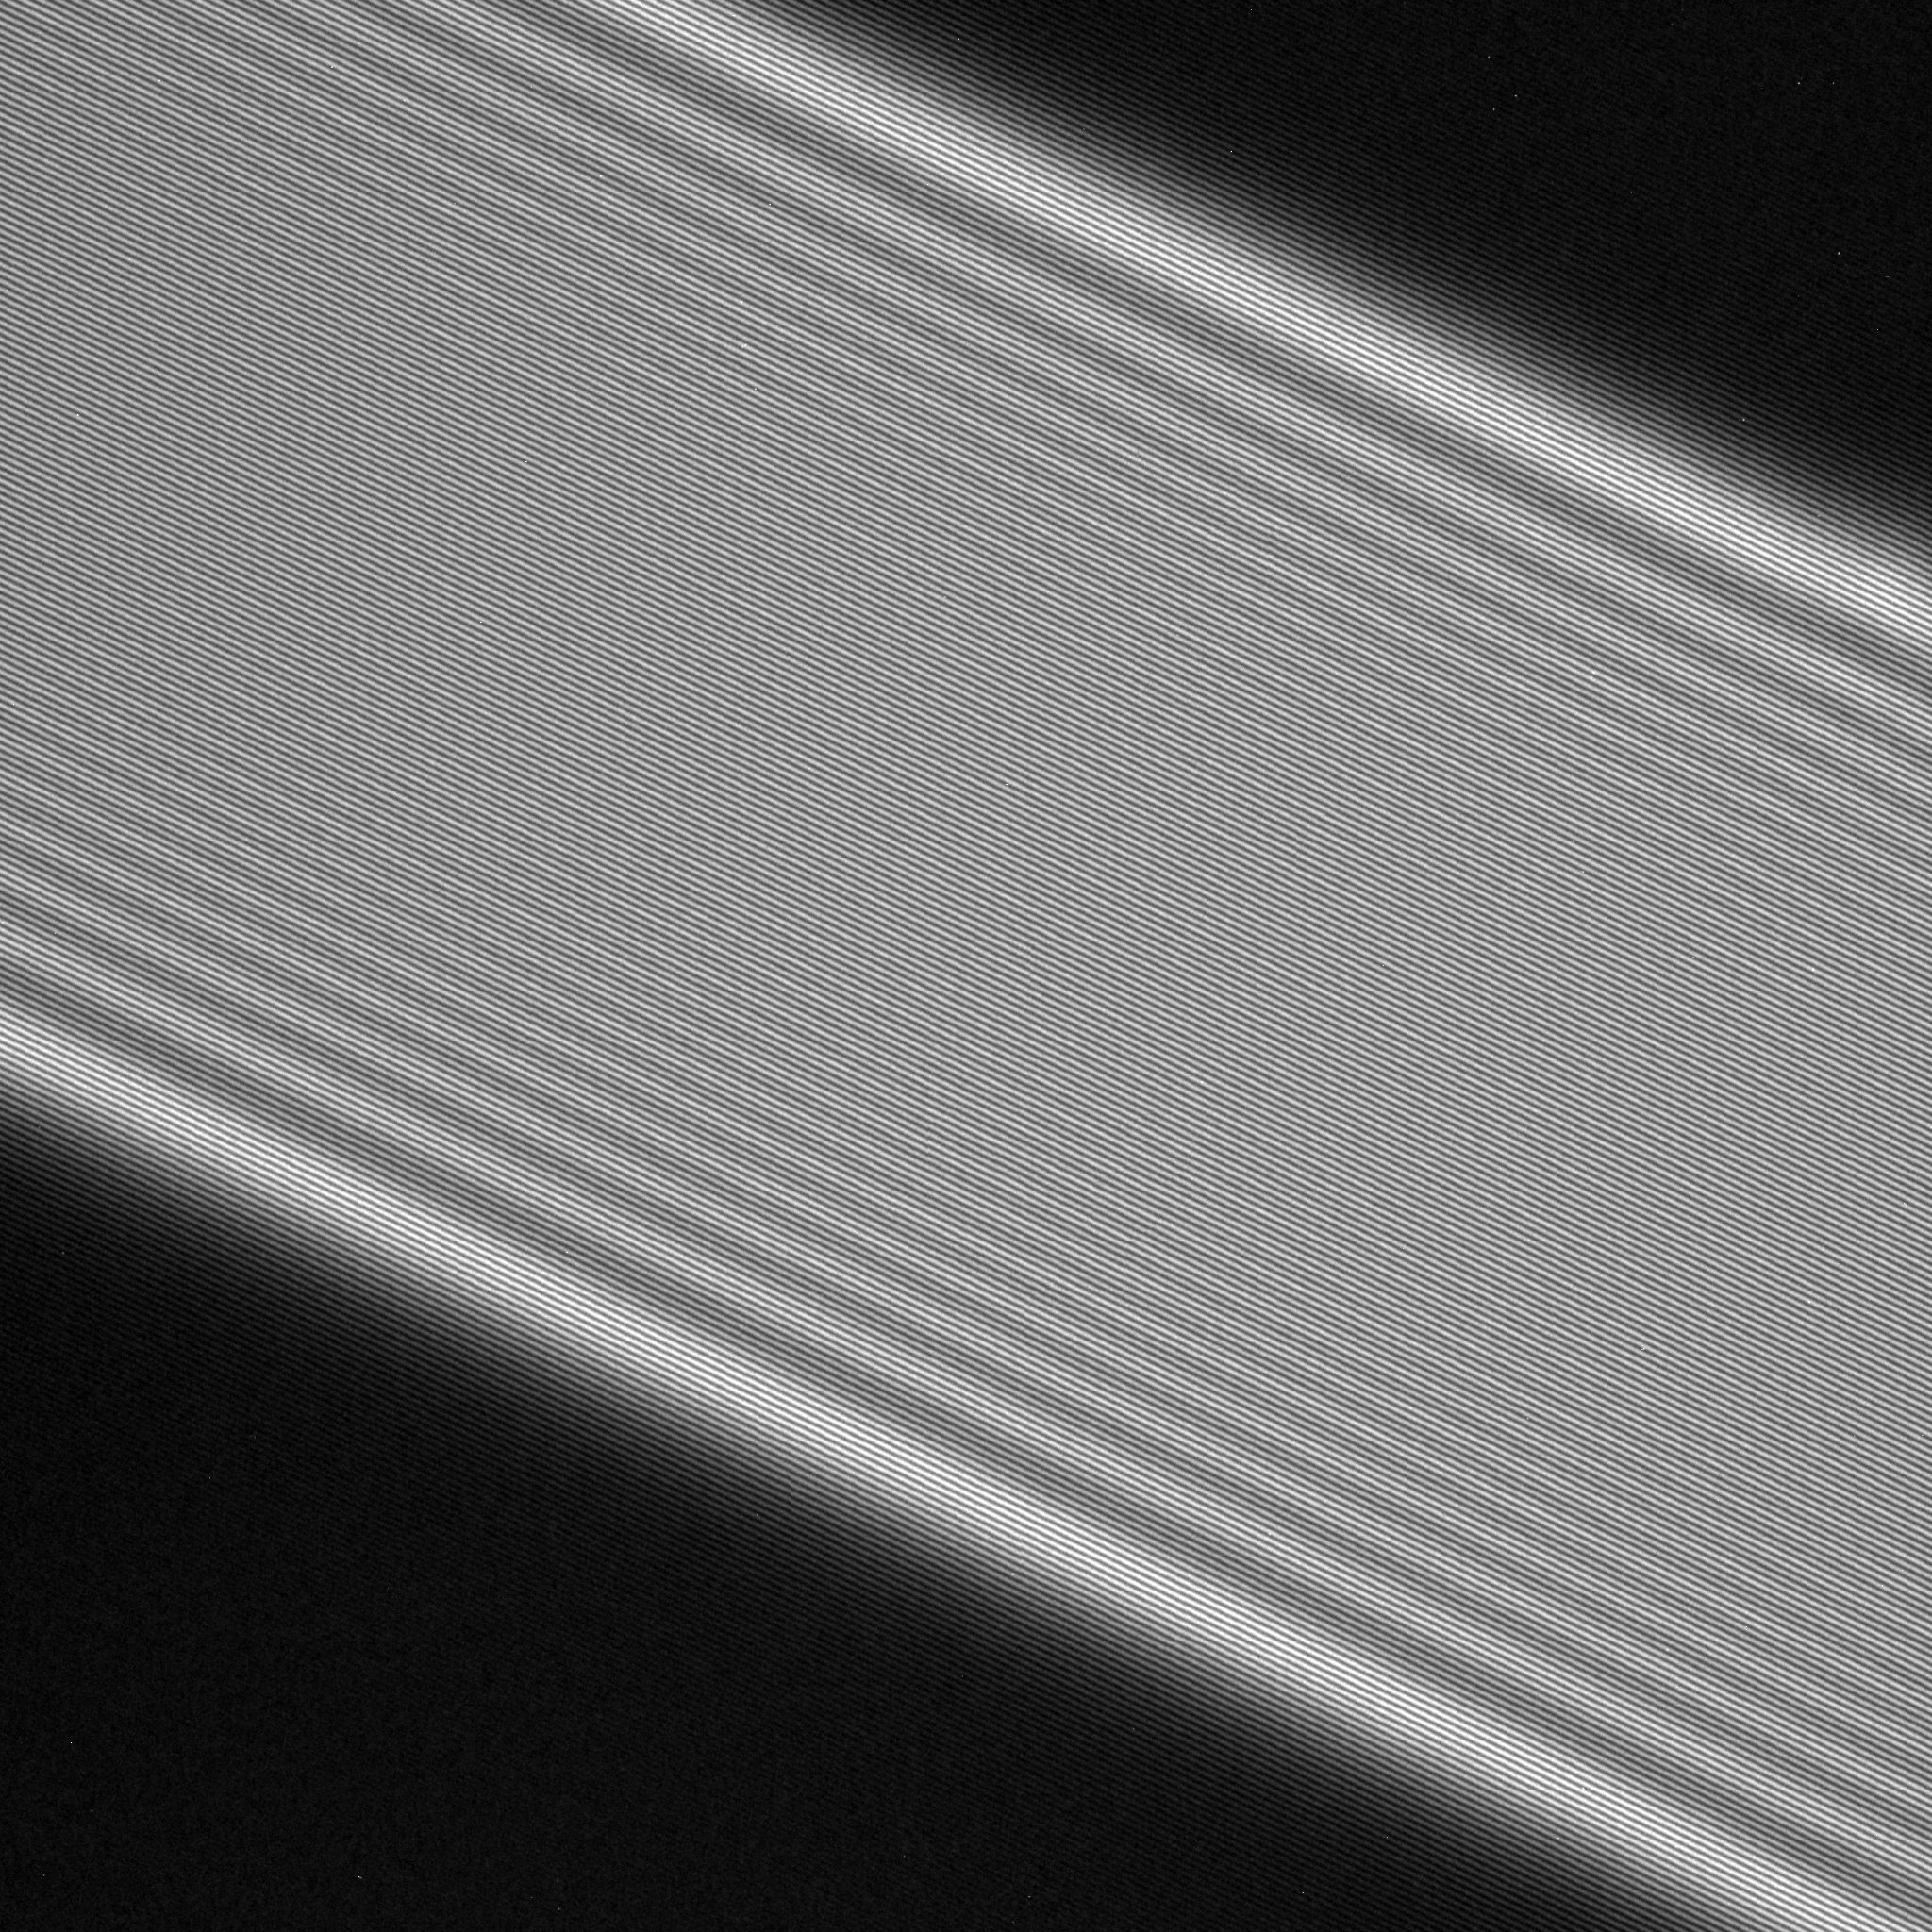
\includegraphics[width=\textwidth]{Holographie/Vakuumhologramm_Elliptischebeleuchtung/60_7_Vak_Ellip.jpg}
         \caption{\(U_F =\) 60,7V}
         \label{604VakEllip}
     \end{subfigure}
     \hfill
     \begin{subfigure}[b]{0.49\textwidth}
         \centering
         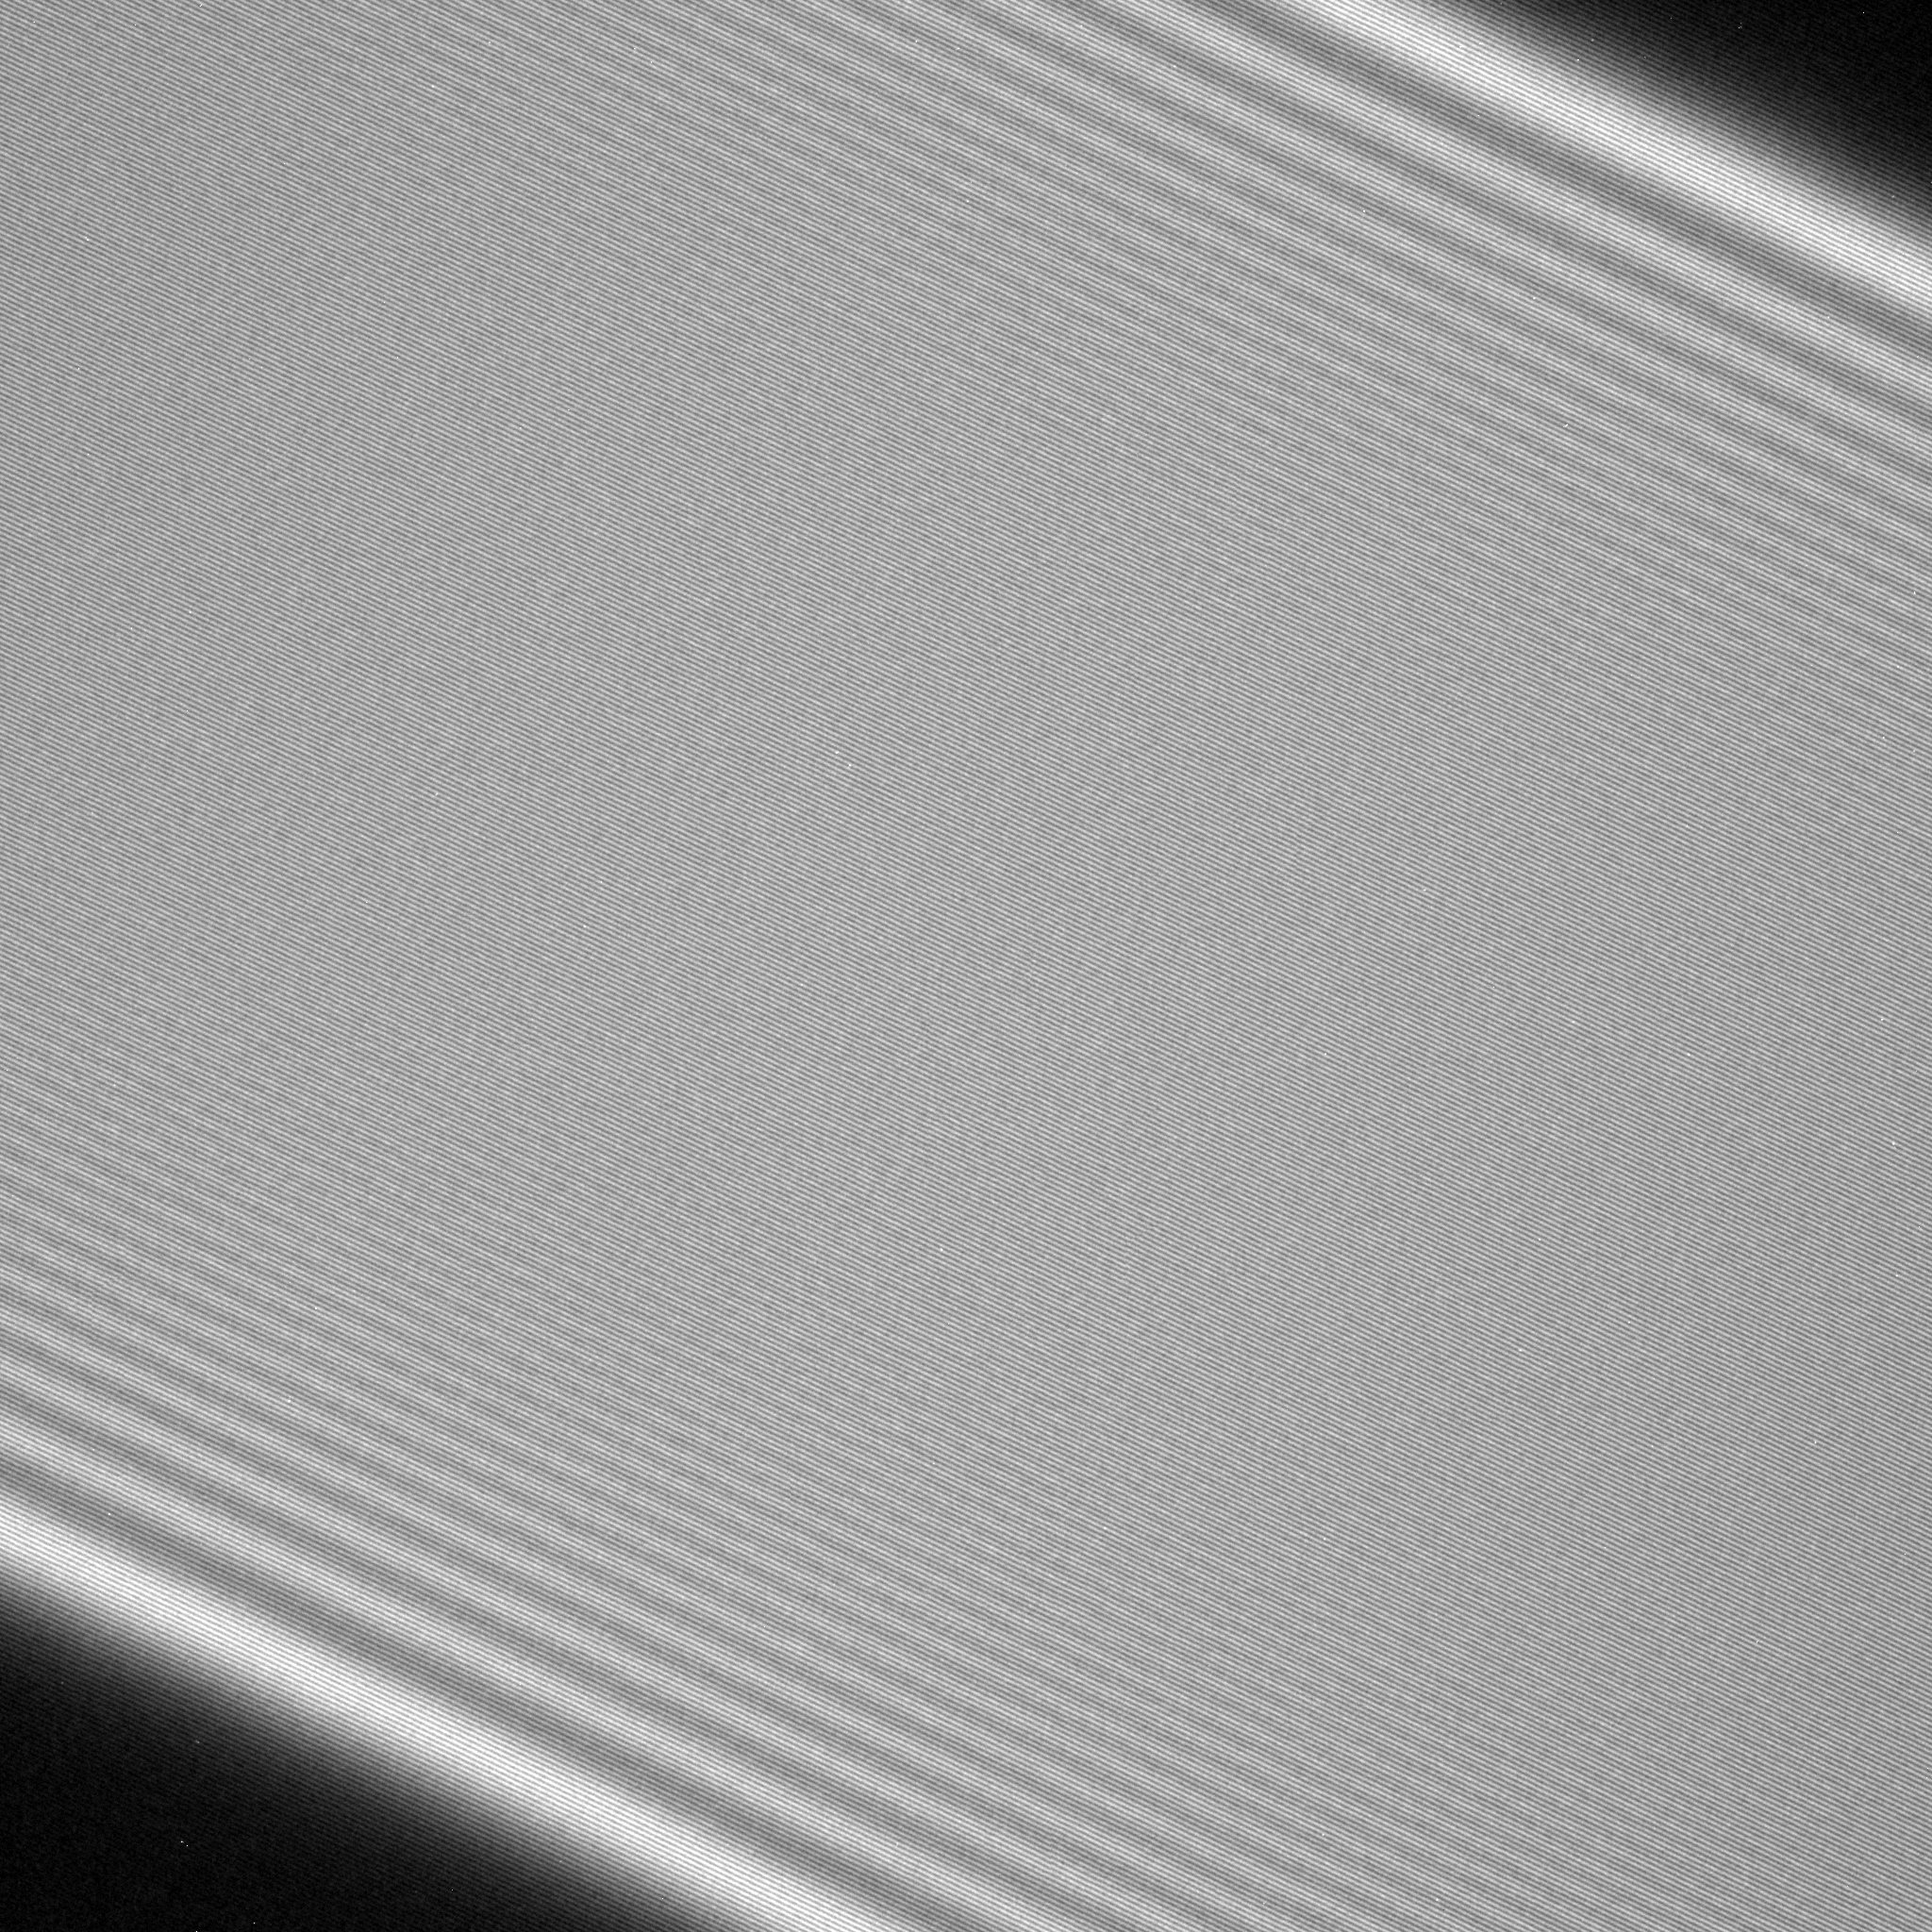
\includegraphics[width=\textwidth]{Holographie/Vakuumhologramm_Elliptischebeleuchtung/89_6_Vak_Ellip.jpg}
         \caption{\(U_F =\) 89,6V}
         \label{896VakEllip}
     \end{subfigure}
     \caption{Leerhologramm mit Elliptischen Beleuchtung bei verschiedenen Fadenspannungen}
        \label{VakHolEllip}
 
\end{figure}

\subsection{P-N Übergang}

Als nächstens wurde eine Silizium Probe untersucht, in der ein P-N Übergang untersucht werden sollte. Zunächst wurde die Probe eingesetzt und nachdem das Vakuum sich stabilisierst hatte wurde das Mikroskop neu eingestellt. Der Probenhalter wurde nun so verkippt das im TEM Modus die Biegekonturen so gering wie möglich erschienen und vor allem in den P-N Übergangsbereich nicht vorhanden waren. Eine Übersichtsaufnahme der Probe ist in Abbildung \cref{P-NÜbersicht} zu sehen, und zwei Aufnahme mit und ohne Biegekonturen im P-N Übergangsbereich sind in Abbildung \cref{P-NOhneKonturen} und \cref{P-NMitKonturen} zu sehn.

\begin{figure}
     \centering
     \begin{subfigure}[b]{0.3\textwidth}
         \centering
         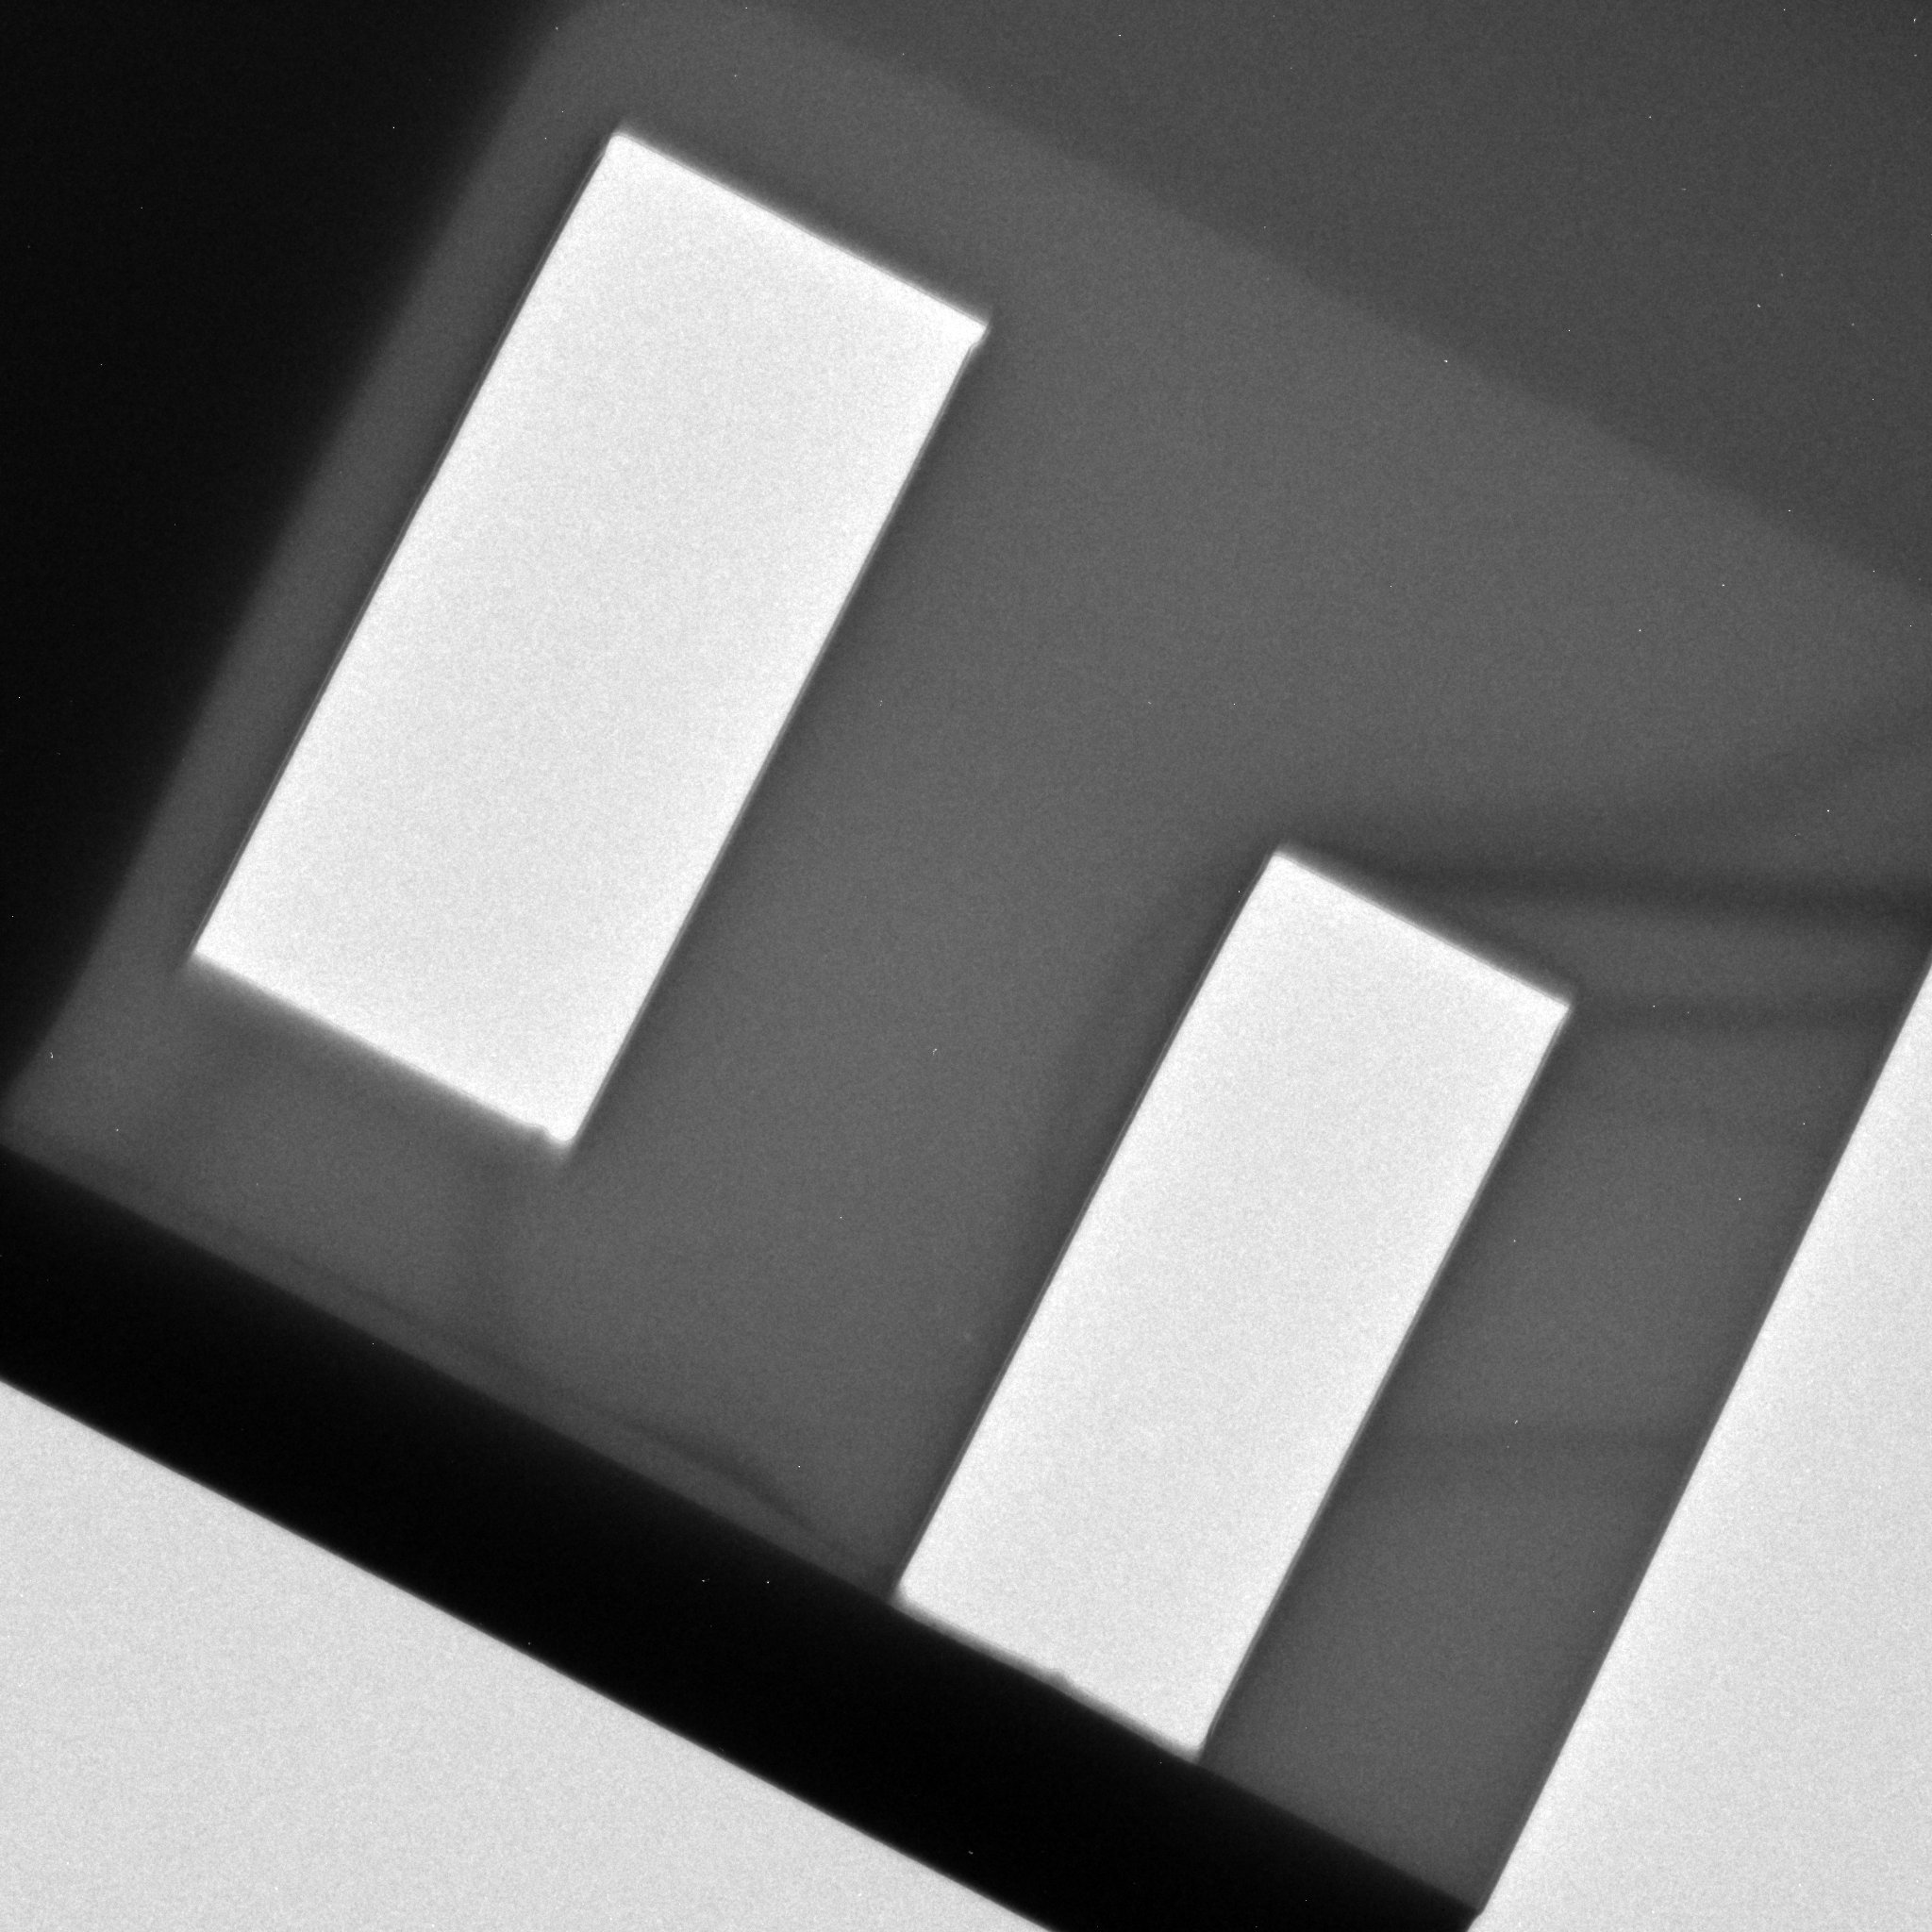
\includegraphics[width=\textwidth]{Holographie/Probe/1_Übersicht1750x_LTZ.jpg}
         \caption{Ganze Probe}
         \label{P-NÜbersicht}
     \end{subfigure}
     \hfill
     \begin{subfigure}[b]{0.3\textwidth}
         \centering
         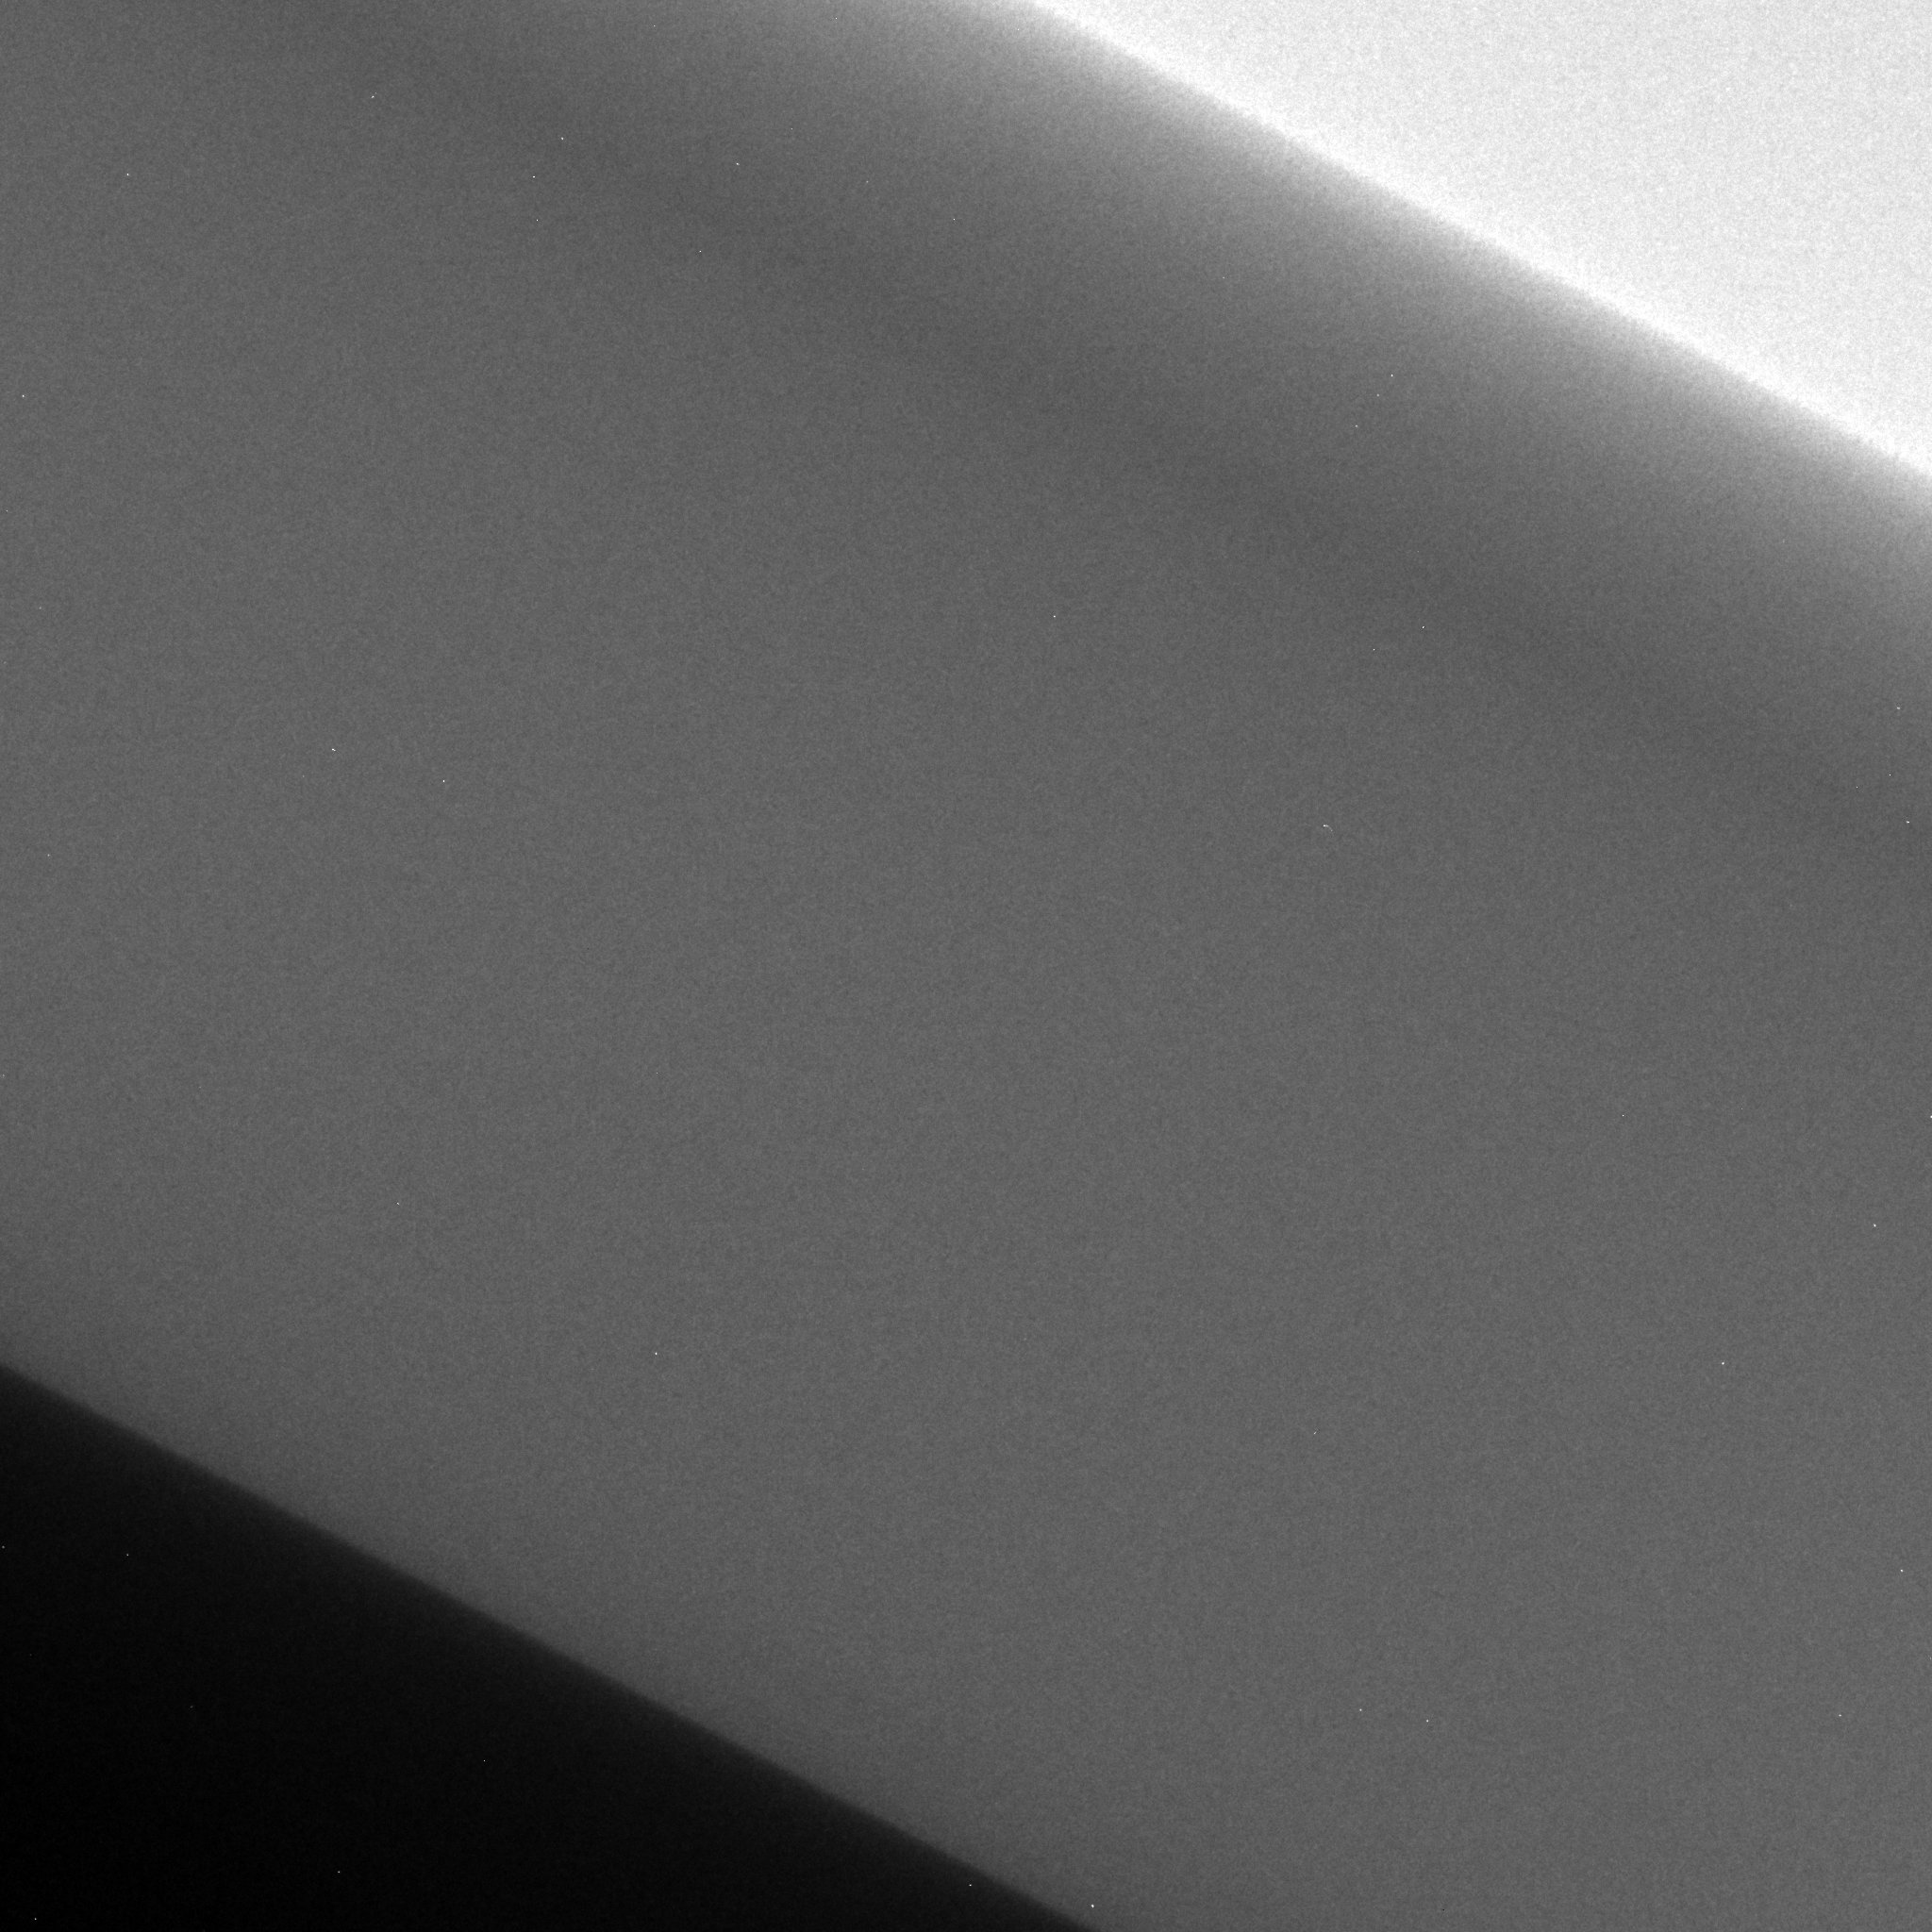
\includegraphics[width=\textwidth]{Holographie/Probe/3_OhneBiegekonuren13500x_LTZ.jpg}
         \caption{P-N Übergang, ohne Biegekonturen.}
         \label{P-NOhneKonturen}
     \end{subfigure}
     \hfill
     \begin{subfigure}[b]{0.3\textwidth}
         \centering
         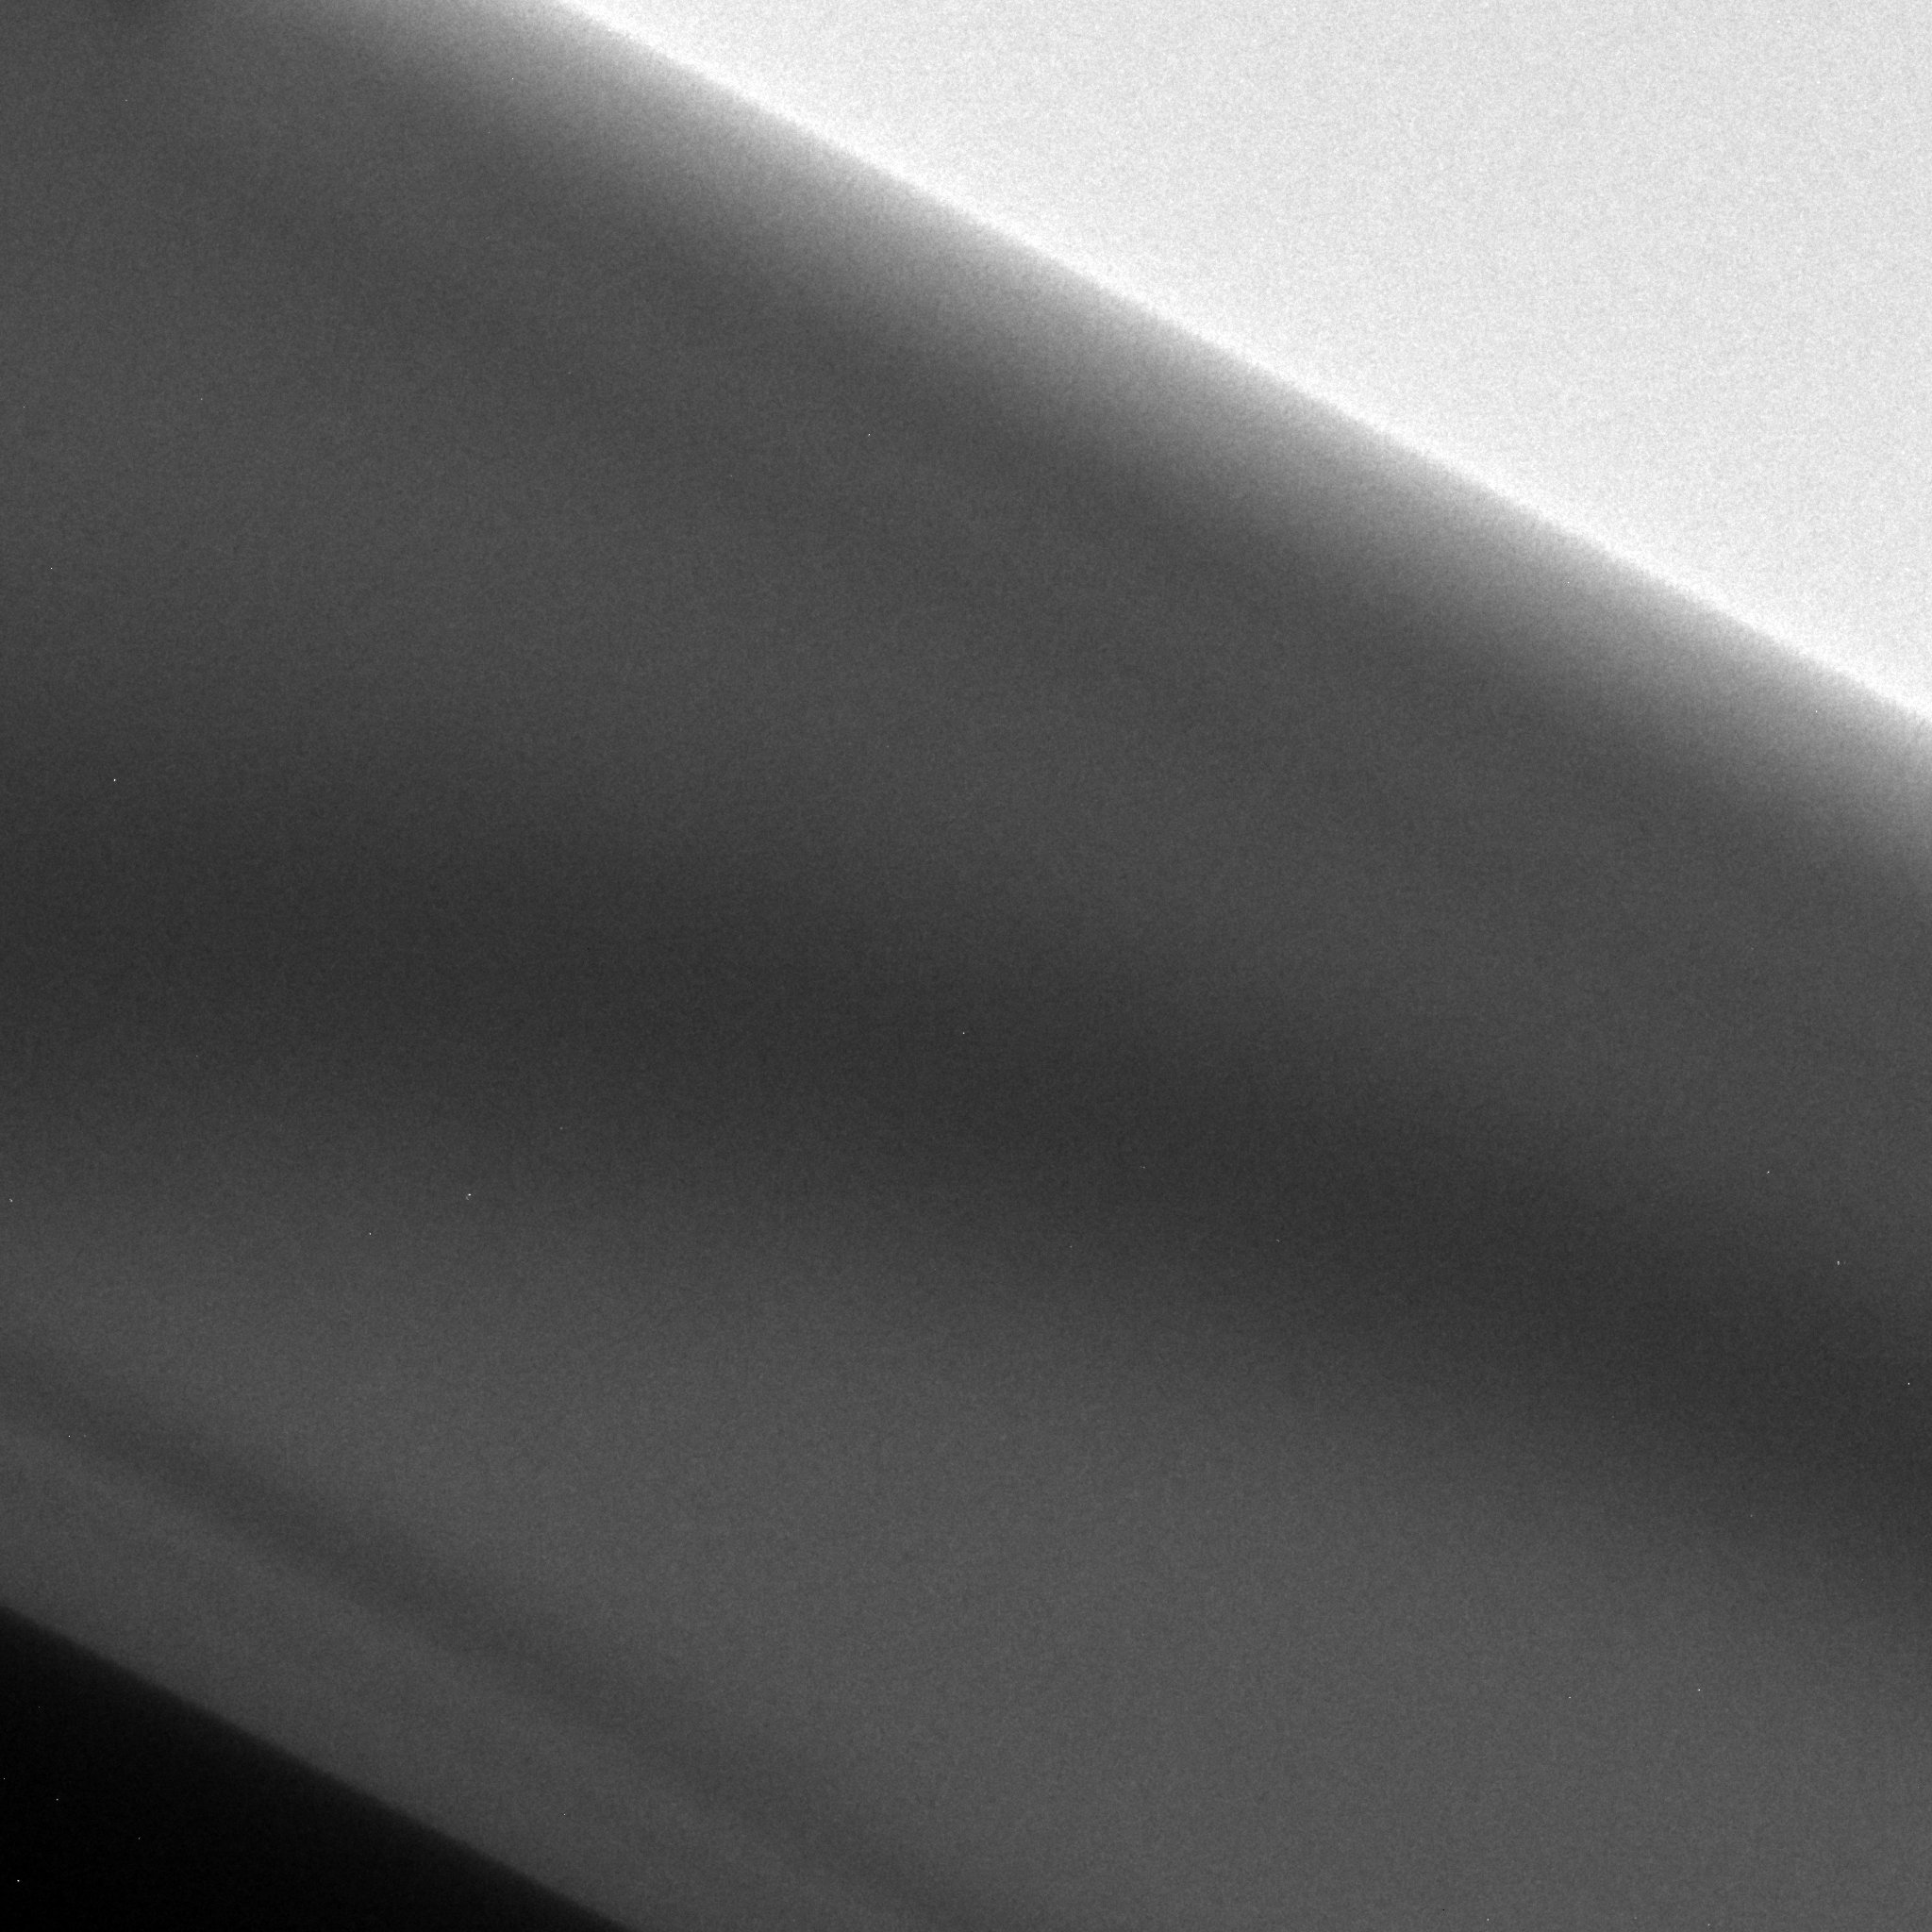
\includegraphics[width=\textwidth]{Holographie/Probe/2_Biegekontur13500x_LTZ.jpg}
         \caption{P-N Übergang, mit Biegekonturen.}
         \label{P-NMitKonturen}
     \end{subfigure}
        \caption{Übersichtsaufnahme der Ganzen Probe (a), und des P-N Übergang (b), (c) mit und ohne Biegekonturen}
        \label{P-NTEMÜbersicht}
\end{figure}

Die Probe wurde so verfahren das das durch die Fokussierte Ionen Dünnung (FIB) erstellte Vakuum Fenster in der Probe so positioniert war das ein Leerhologramm durch das Fenster erstellt werden konnte. Dabei wurde eine Rundbeleuchtung verwendet und eine Fadenspannung von 70V. Abbildung \cref{P-NLeer}\\
Anschließen wurde die Probe so verfahren das sich der Biprisma Faden an der Kante des festeres befand, um nun zwei gut separate Teilwellen für das Hologramm erhalten zu können. Hier wurde eine Hologramm Aufnahme erstelle, bei der die Mikroskope Einstellungen des Leer Hologramm beibehalten wurden. Das Hologramm ist in Abbildung \cref{P-NObjekt} zu sehen.\\
Die Messungen wurden analog zur rund Beleuchtung mit einer elliptischen Beleuchtung wiederholt.

\begin{figure}[H]
     \centering
     \begin{subfigure}[b]{0.49\textwidth}
         \centering
         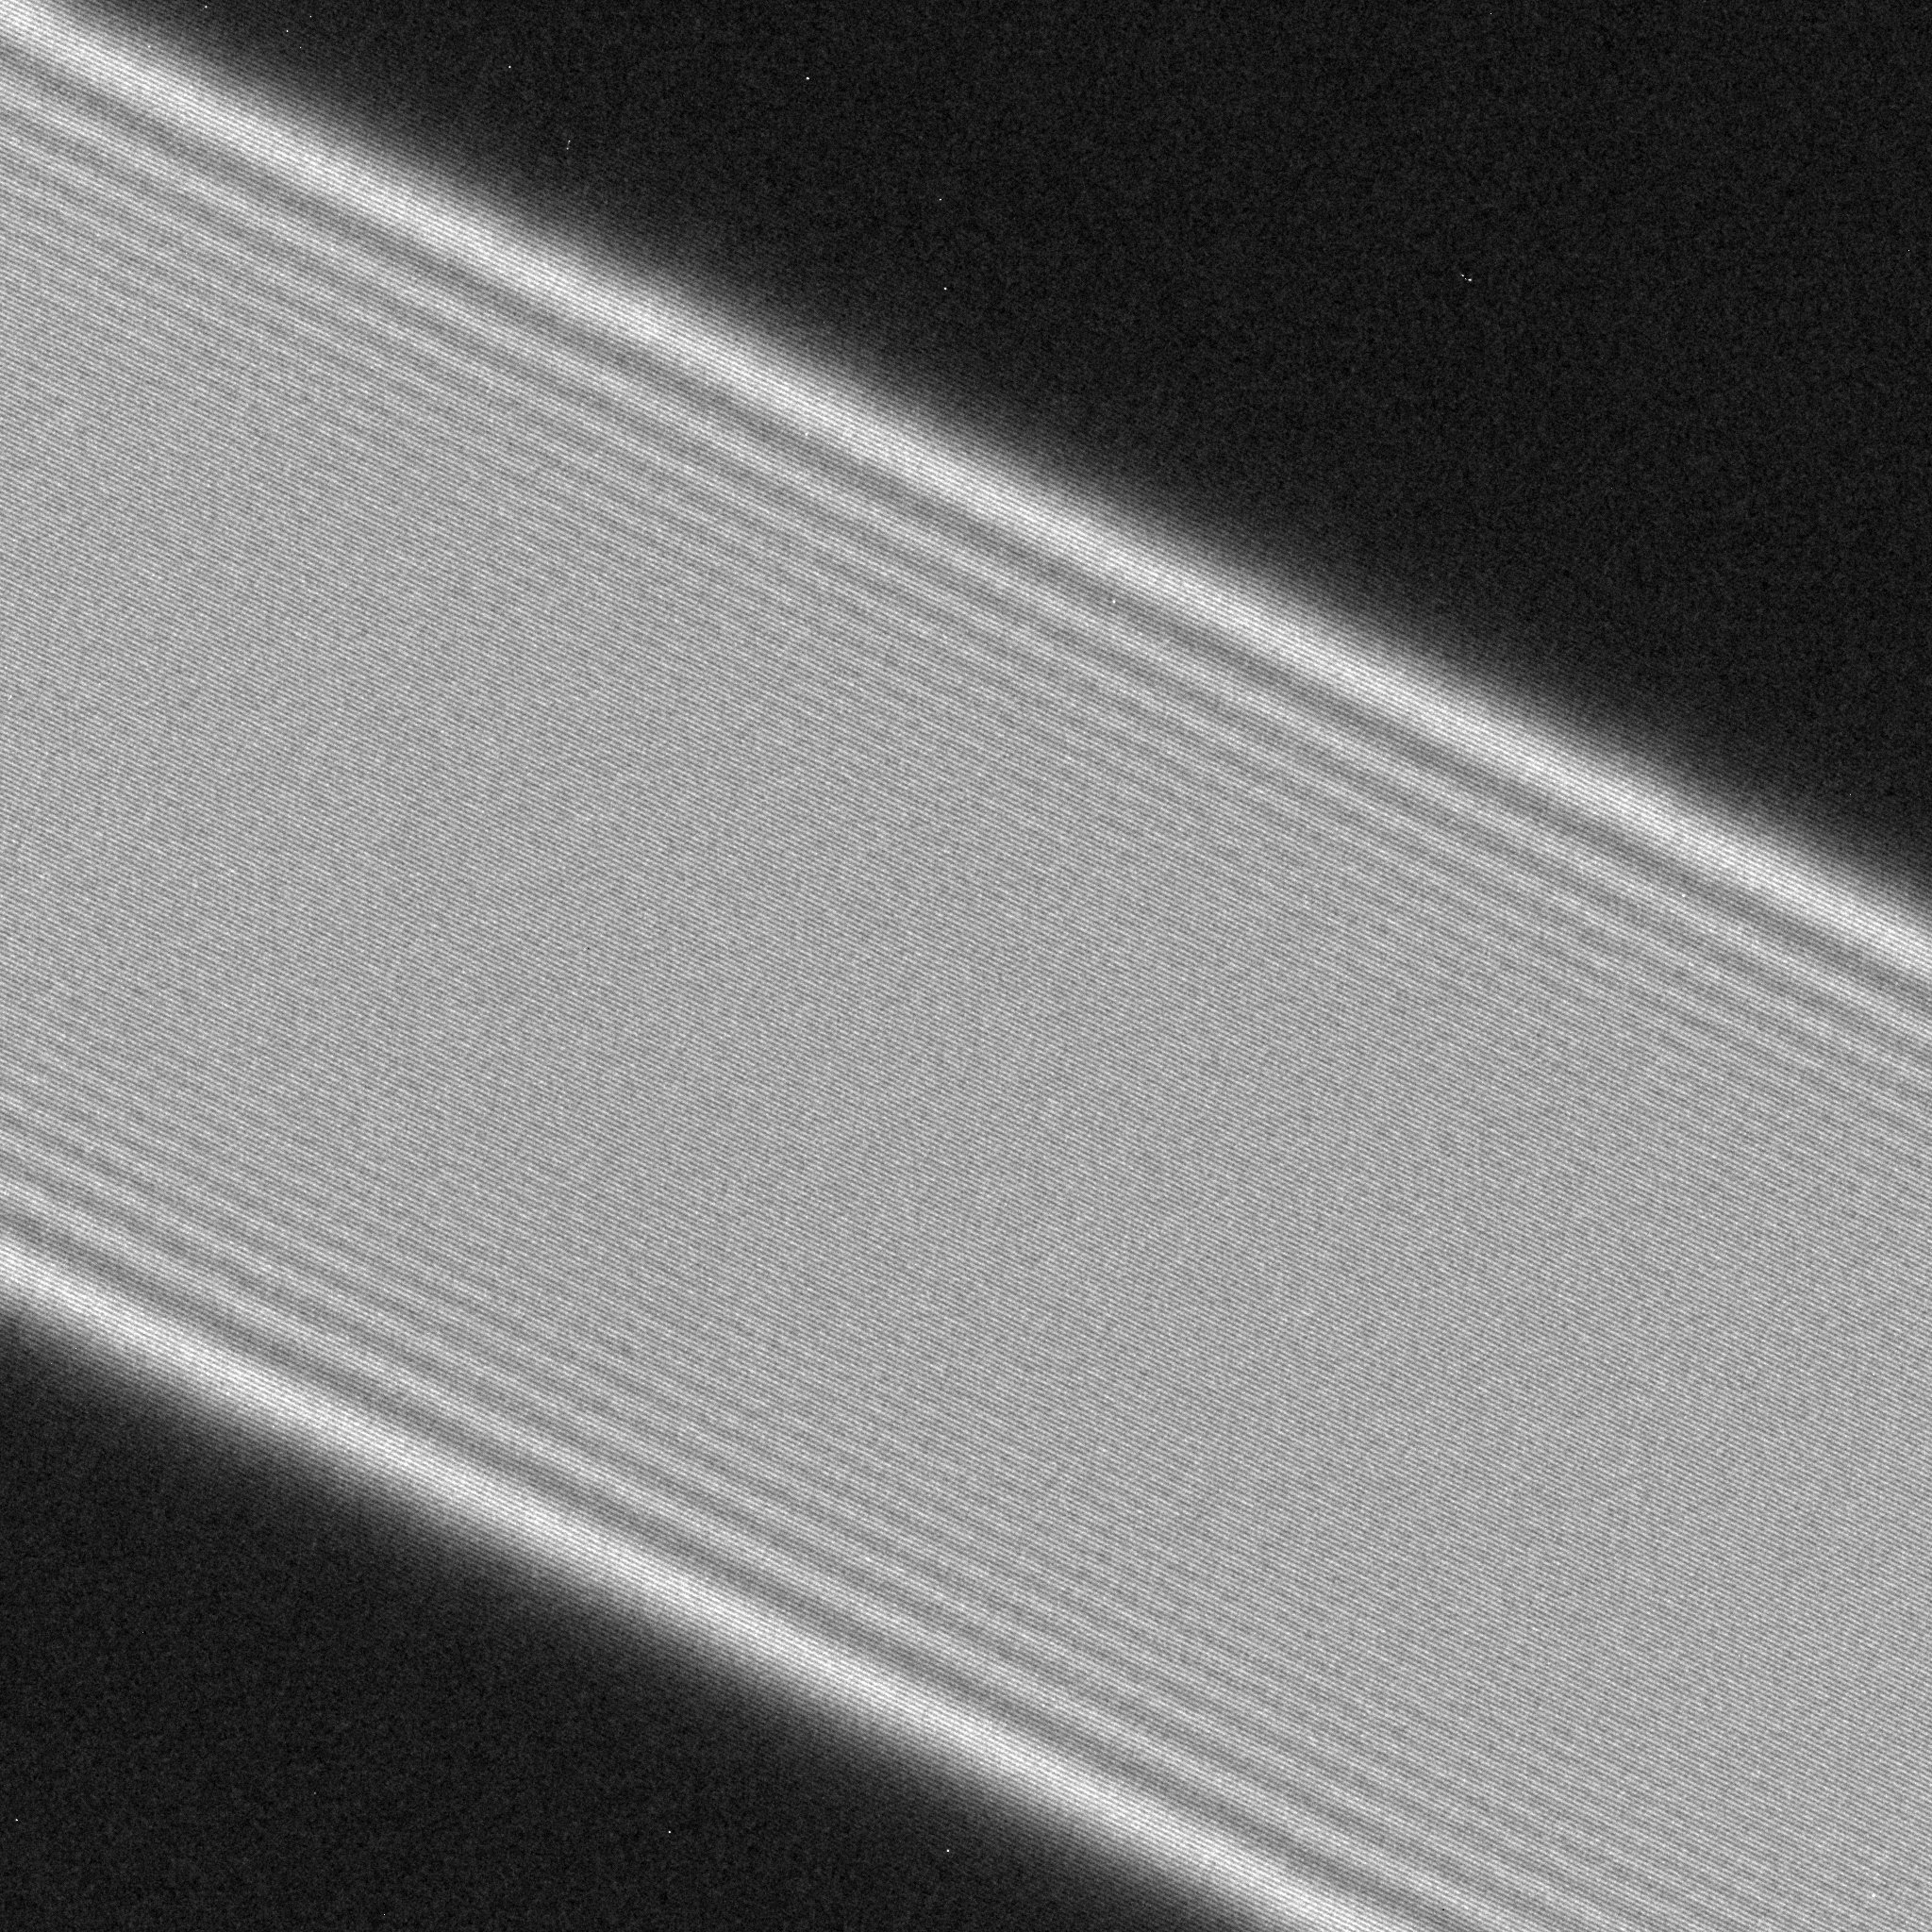
\includegraphics[width=\textwidth]{Gerüst/Abbildungen/Holographie/Probe/4_Rundbeleuchtung_Hologram_15500x_LTZ.jpg}
         \caption{Leerhologramm}
         \label{P-NLeer}
     \end{subfigure}
     \hfill
     \begin{subfigure}[b]{0.49\textwidth}
         \centering
         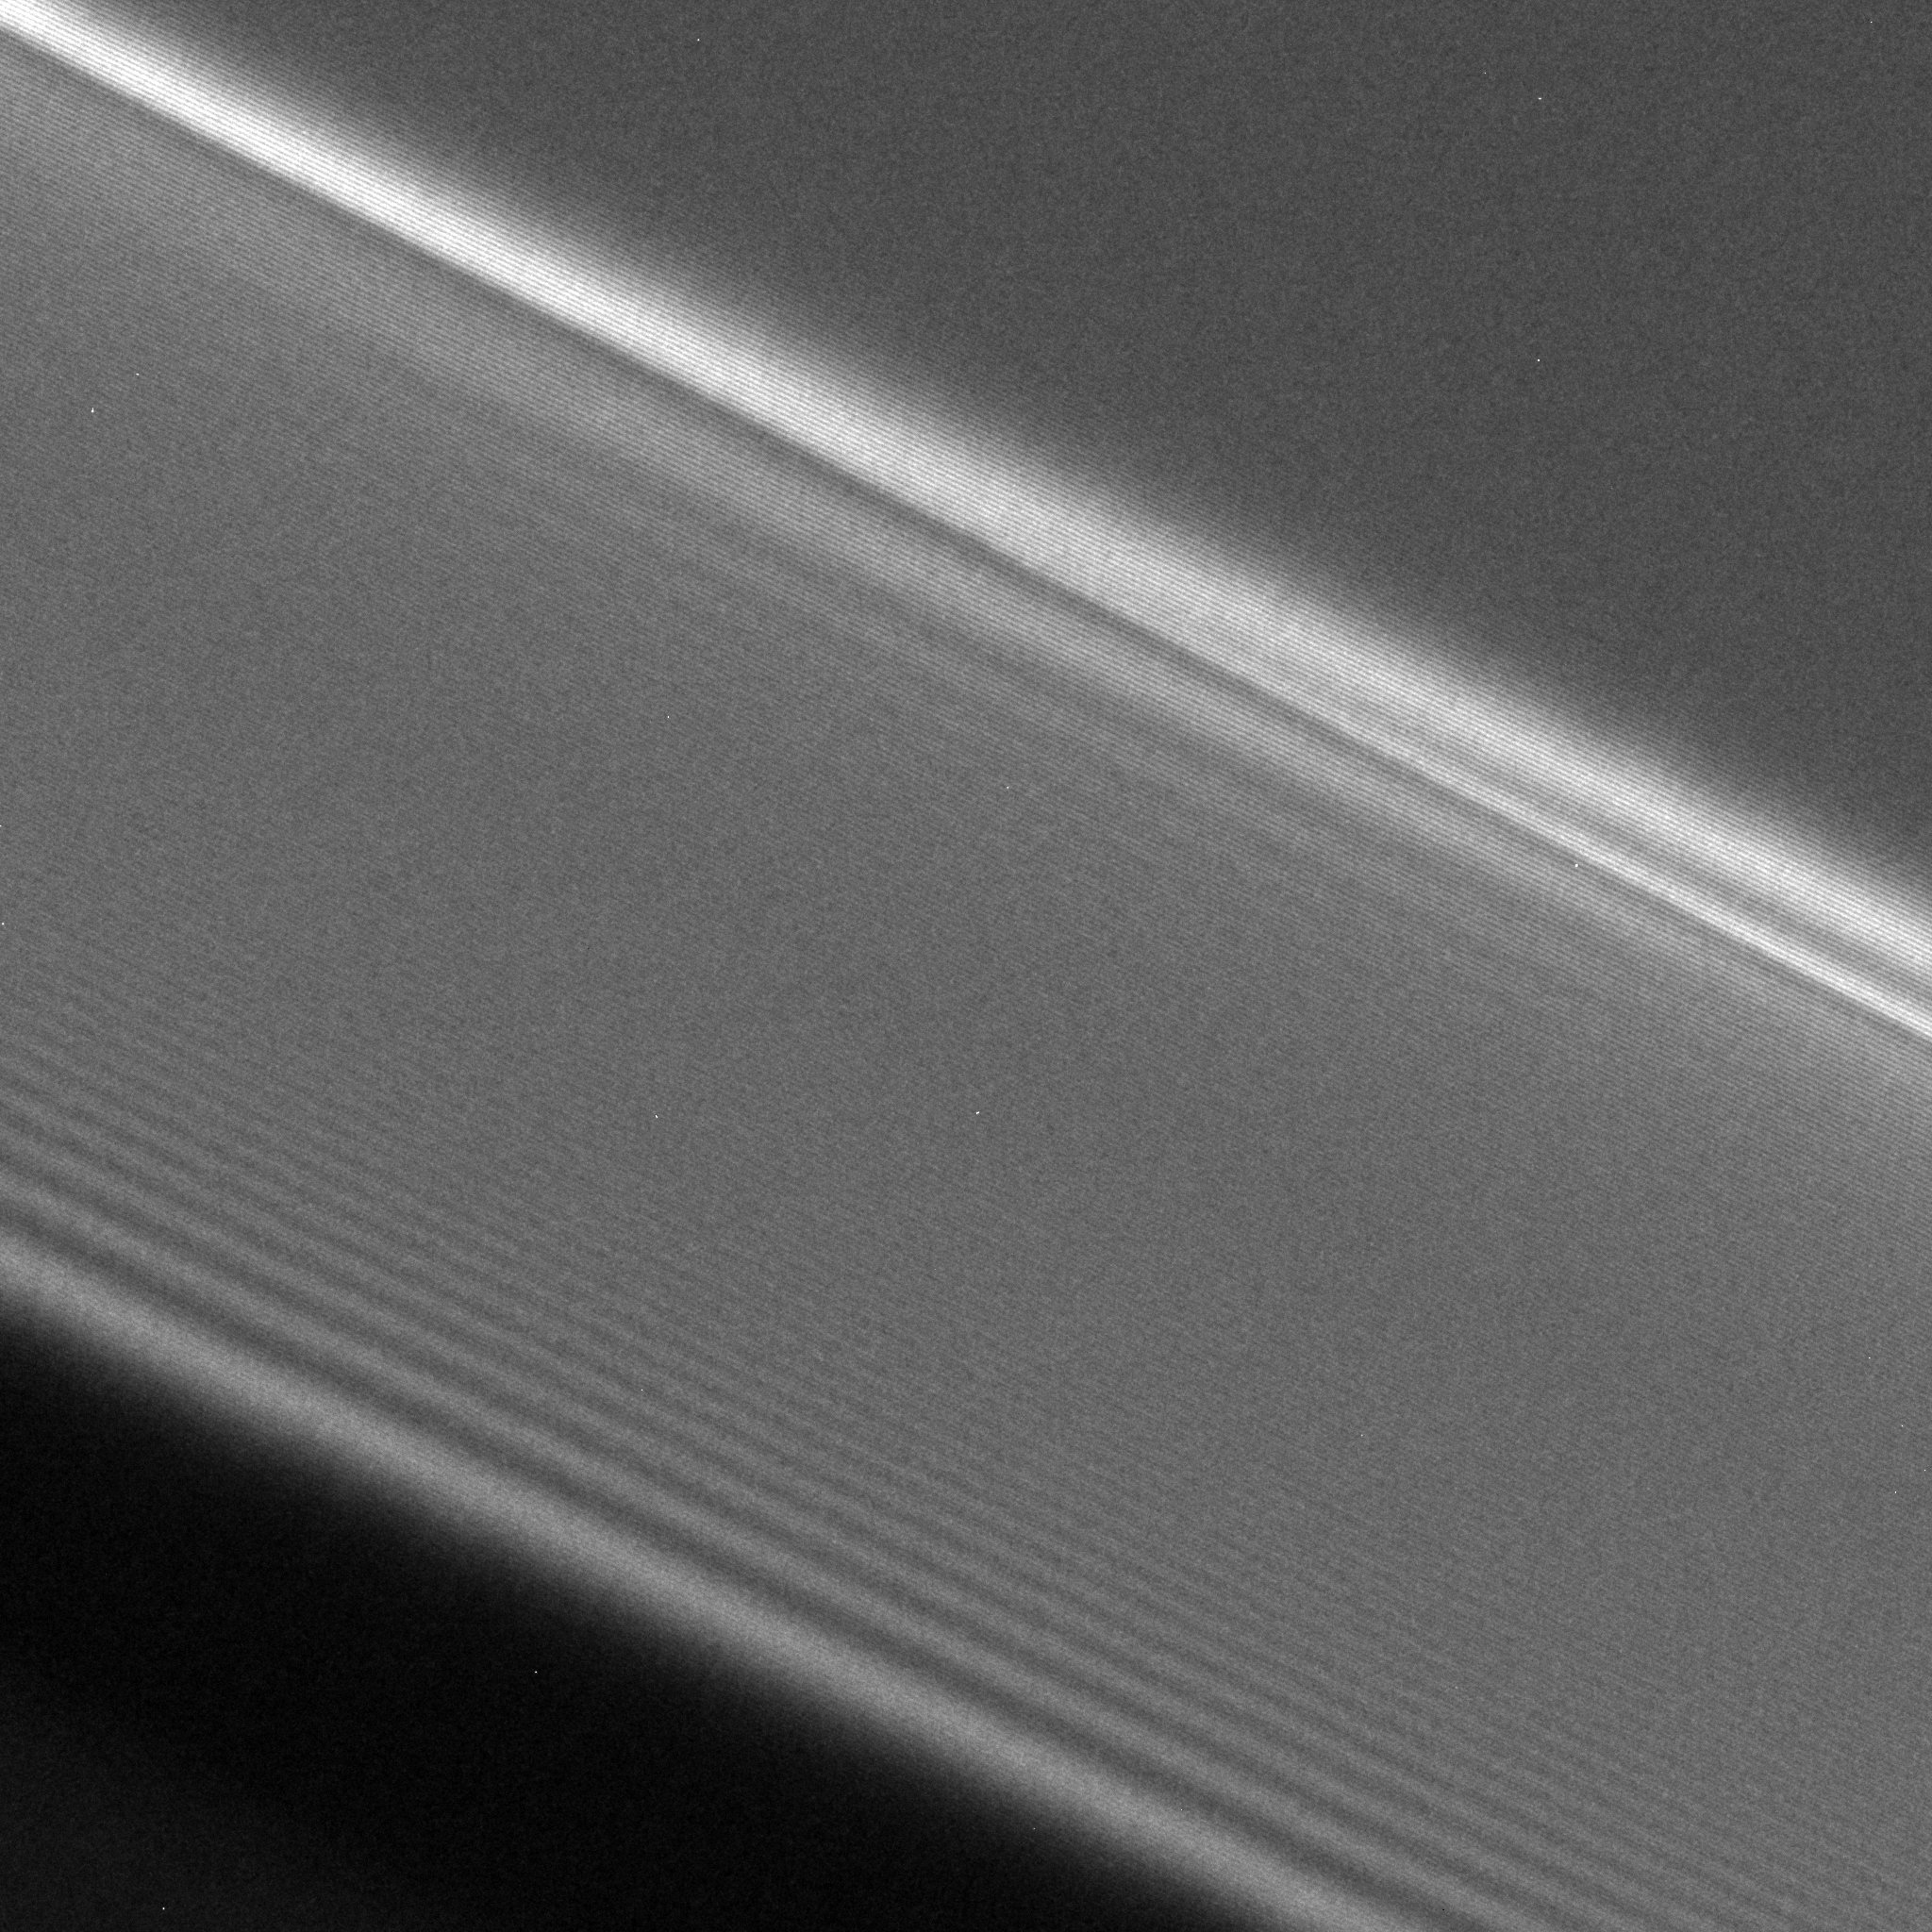
\includegraphics[width=\textwidth]{Gerüst/Abbildungen/Holographie/Probe/5_Rundbeleuchtung_Hologram_an_derKante_15500x_LTZ.jpg}
         \caption{Objekthologramm}
         \label{P-NObjekt}
     \end{subfigure}
        \caption{Hologramm Aufnahme von Silizum Chip mit P-N Übergang}
        \label{AmpPhaseBild}
\end{figure}

\subsubsection{Rekonstruktion des Hologramms}

Um aus dem Hologramm die Phasen und Amplitudeninformation zu erhalten, muss man die komplexe bildwelle rekonstruieren. Hierfür wird zunächst eine Fast Fourier Transformation aus dem Hologramm erstellt. Dabei entsteht eine Komplexes Fourier Spektrum. In diesem Fourier Spektrum ist das Zentralband mit zwei Seiten Bänder (Seitenband -1 und Seitenband +1) abgebildet.\\
Zur Rekonstruktion wird das Seitenband +1 verwendet, dies ist das das Vakuum seitige band. Dieses Band wird ausgeschnitten und zentriert um es anschließend Inverse Fourier zu transformieren. Dadurch wird die Komplexe Bildwelle erstellt.

\subsubsection{Leerhologramm und Korrektur}

Um die Qualität der Bildwelle zu verbessern kann ein Leerhologramm verwendet werden, dadurch kann die verzeichnungsbedingte Phasenmodulation korrigieren werden. Die Korrektur wird erreicht, wenn die bei der Rekonstruktion erhaltene Bildwelle durch die Vakuum Bildwelle geteilt wird. Dabei werden die Amplituden miteinander geteilt und die Phasen voneinander abgezogen. Als Resultat erhält man nun ein korrigiertes Phasen und Amplitudenbild.

\subsubsection{Auswertung}

Im Amplitudenbild mit der rund Beleuchtung Abbildung \cref{P-NAmp} ist der P-N Übergang nicht erkennbar es ist lediglich die Kante zum Vakuum (Oben Rechts) erkennbar. \\
Beim dem Phasenbild ist der P-N Übergang wesentlich besser zu erkenn, siehe Abbildung \cref{P-NPhaseW} (Wrappt), es ist hier ein klarer Kontrast erkennbar der etwas unter der Kante zum Vakuum liegt. Sowie bei dem durch dem Goldsted Algorithmus Bearbeitetem (Unwraped) Phasenbild \cref{P-NphaseU}. 

\begin{figure}
     \centering
     \begin{subfigure}[b]{0.3\textwidth}
         \centering
         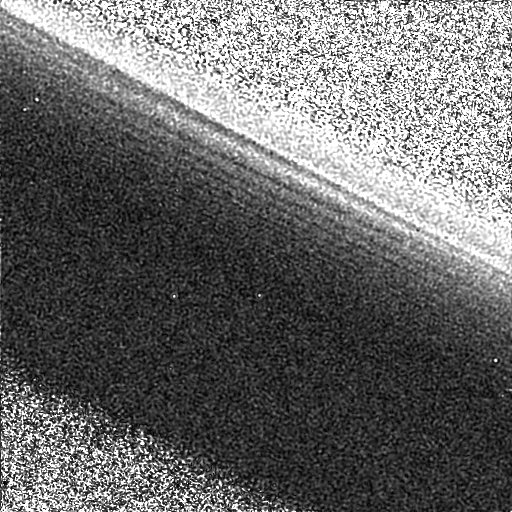
\includegraphics[width=\textwidth]{Holographie/Probe/6_Rundbeleuchtung_amplitude_keil.jpg}
         \caption{Amplitudenbild}
         \label{P-NAmp}
     \end{subfigure}
     \hfill
     \begin{subfigure}[b]{0.3\textwidth}
         \centering
         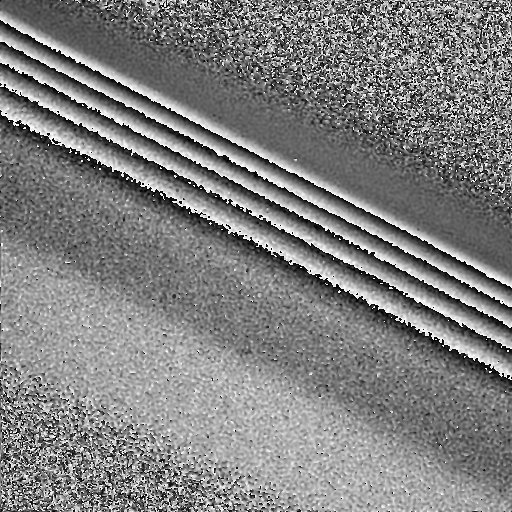
\includegraphics[width=\textwidth]{Holographie/Probe/7_Rundbeleuchtung_Unkorigirten_Phase_über_ort_15500x_LTZ.jpg}
         \caption{Phasenbild, Wrapped}
         \label{P-NPhaseW}
     \end{subfigure}
     \hfill
     \begin{subfigure}[b]{0.3\textwidth}
         \centering
         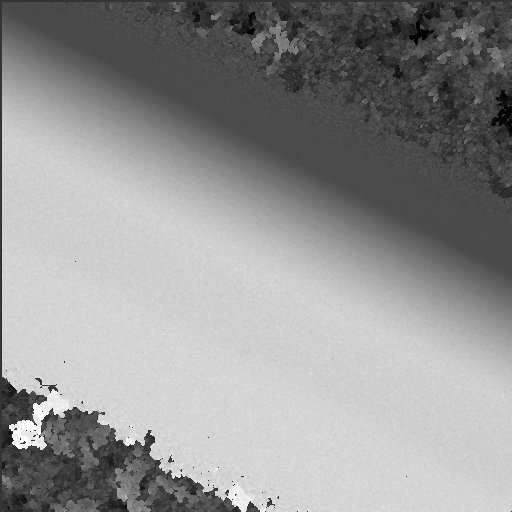
\includegraphics[width=\textwidth]{Holographie/Probe/8_Rundbeleuchtung_Korrigiert_Unwraptbild_15500x_LTZ.jpg}
         \caption{Phasenbild, Unwrapped}
         \label{P-NphaseU}
     \end{subfigure}
        \caption{}
        \label{P-NTEMÜber}
\end{figure}

Die Unwrapped Phasenkeil Aufnahme kann verwendet werden um die Dicke der Probe zu bestimmen dabei wird die Phasen Schiebung im Phasenkeil im Grapf \cref{P-NKeil} ausgewertet. Dabei kann abgelesen werden das die Phasenschiebung im Keil \(30 rad\) beträgt, wenn nun die Funktion \cref{eq:PhaseShift} zur Hilfe genommen wird kann die Dicke der Probe bestimmt werden. Hierbei wird das mittleres inneres potential, \(V^{Si}_{MIP} = 12.57V\) verwendet, um eine Objektdicke von \(350nm\) zu berechnet.

\begin{figure}[H]
     \centering
     \begin{subfigure}[b]{0.49\textwidth}
         \centering
         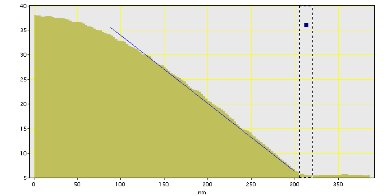
\includegraphics[width=\textwidth]{Gerüst/Abbildungen/Holographie/Probe/8_Rundbeleuchtung_Lieniendiagram_keil.jpg}
         \caption{Phasenkeil}
         \label{P-NKeil}
     \end{subfigure}
     \hfill
     \begin{subfigure}[b]{0.49\textwidth}
         \centering
         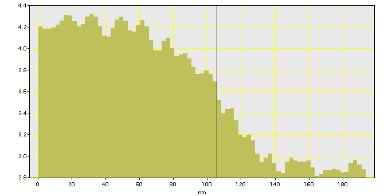
\includegraphics[width=\textwidth]{Gerüst/Abbildungen/Holographie/Probe/8_Rundbeleuchtung_Lieniendiagram_PN_übergang.jpg}
         \caption{P-N Übergang}
         \label{P-NPhase}
     \end{subfigure}
        \caption{Graph der Phasenschiebung des phasenkeil im Unwarapped Phasenbild (quer über den Keil gemessen) und des P-N Übergang um Wrapped Phasenbild (quer über den Übergang gemessen)}
        \label{P-NDiagram}
\end{figure}

In der unkorrigierten (Wrapped) Aufnahme ist ein Kontrast des P-N Übergang erkennbar, dieser entspricht der Phasenschiebung der durch das unterschiedlichen Elektrische Potential im P-N Übergang verursacht wird. Die Phasenschiebung im P-N Übergang ist im Graph \cref{P-NPhase} ausgewertet und beträgt \(1,4 rad\). Die Dotierung kann nun mit Hilfe von \cref{eq:PhaseShift} und dem zuvor berechnenden Objektdicke berechnend werden und beträgt \(1*10^-19 cm^{-2}\) Anzahl gedopte Atome pro \(cm^{-2}\).\\
Zuletzt wurde Phasenbild mit Hilfe der Mikroskopie Software die breite des P-N Übergang bestimmt, welche \(80 nm\) beträgt.\\
Diese Auswertung wurde nicht mit der elliptischen Beleuchtung wiederholt die Hologramm aufnahmen und Amplituden-/Phasenbilder sind jedoch in Abbildung \cref{P-NHologrammEllip} und \cref{AmpPhaseBildEllip} zu sehen. Es ist ein besserer Kontrast bei den Aufnahmen mit der elliptischen Beleuchtung zu beobachten.

\begin{figure}[H]
     \centering
     \begin{subfigure}[b]{0.49\textwidth}
         \centering
         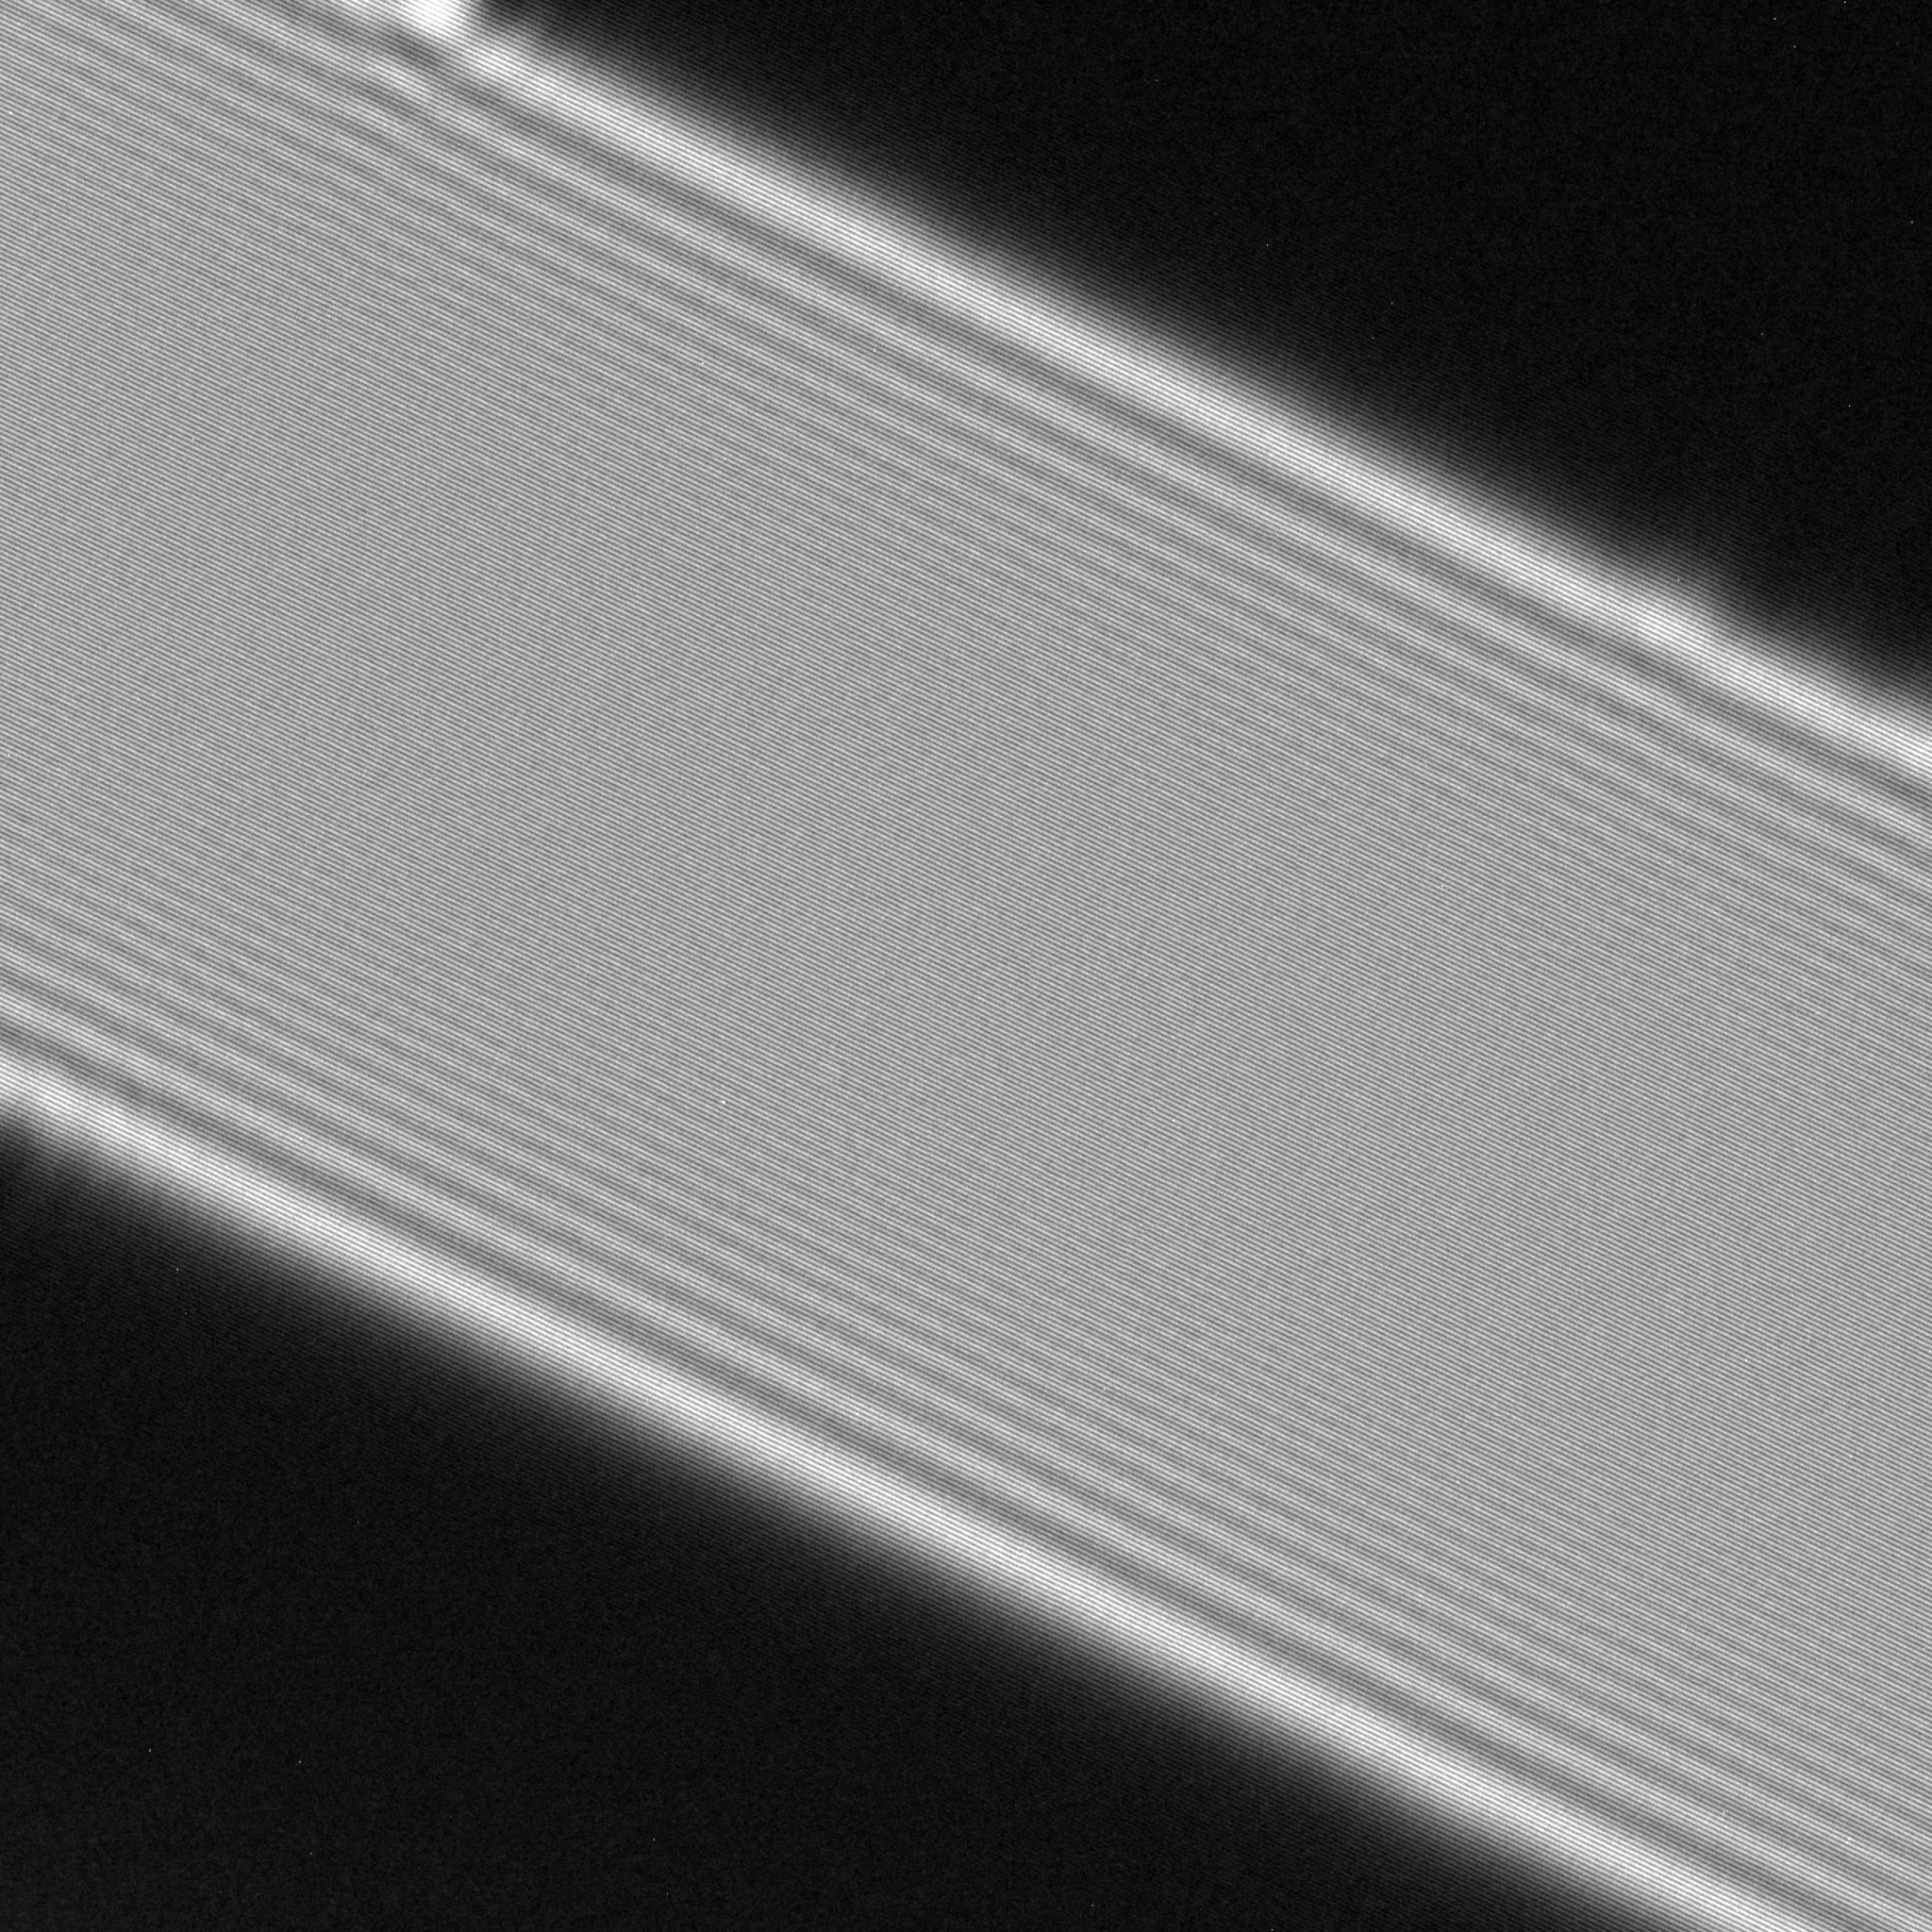
\includegraphics[width=\textwidth]{Gerüst/Abbildungen/Holographie/Probe/1_Leerhologramm_70.4V_Ltz_15500x.jpg}
         \caption{Leerhologramm}
         \label{P-NLeerEllip}
     \end{subfigure}
     \hfill
     \begin{subfigure}[b]{0.49\textwidth}
         \centering
         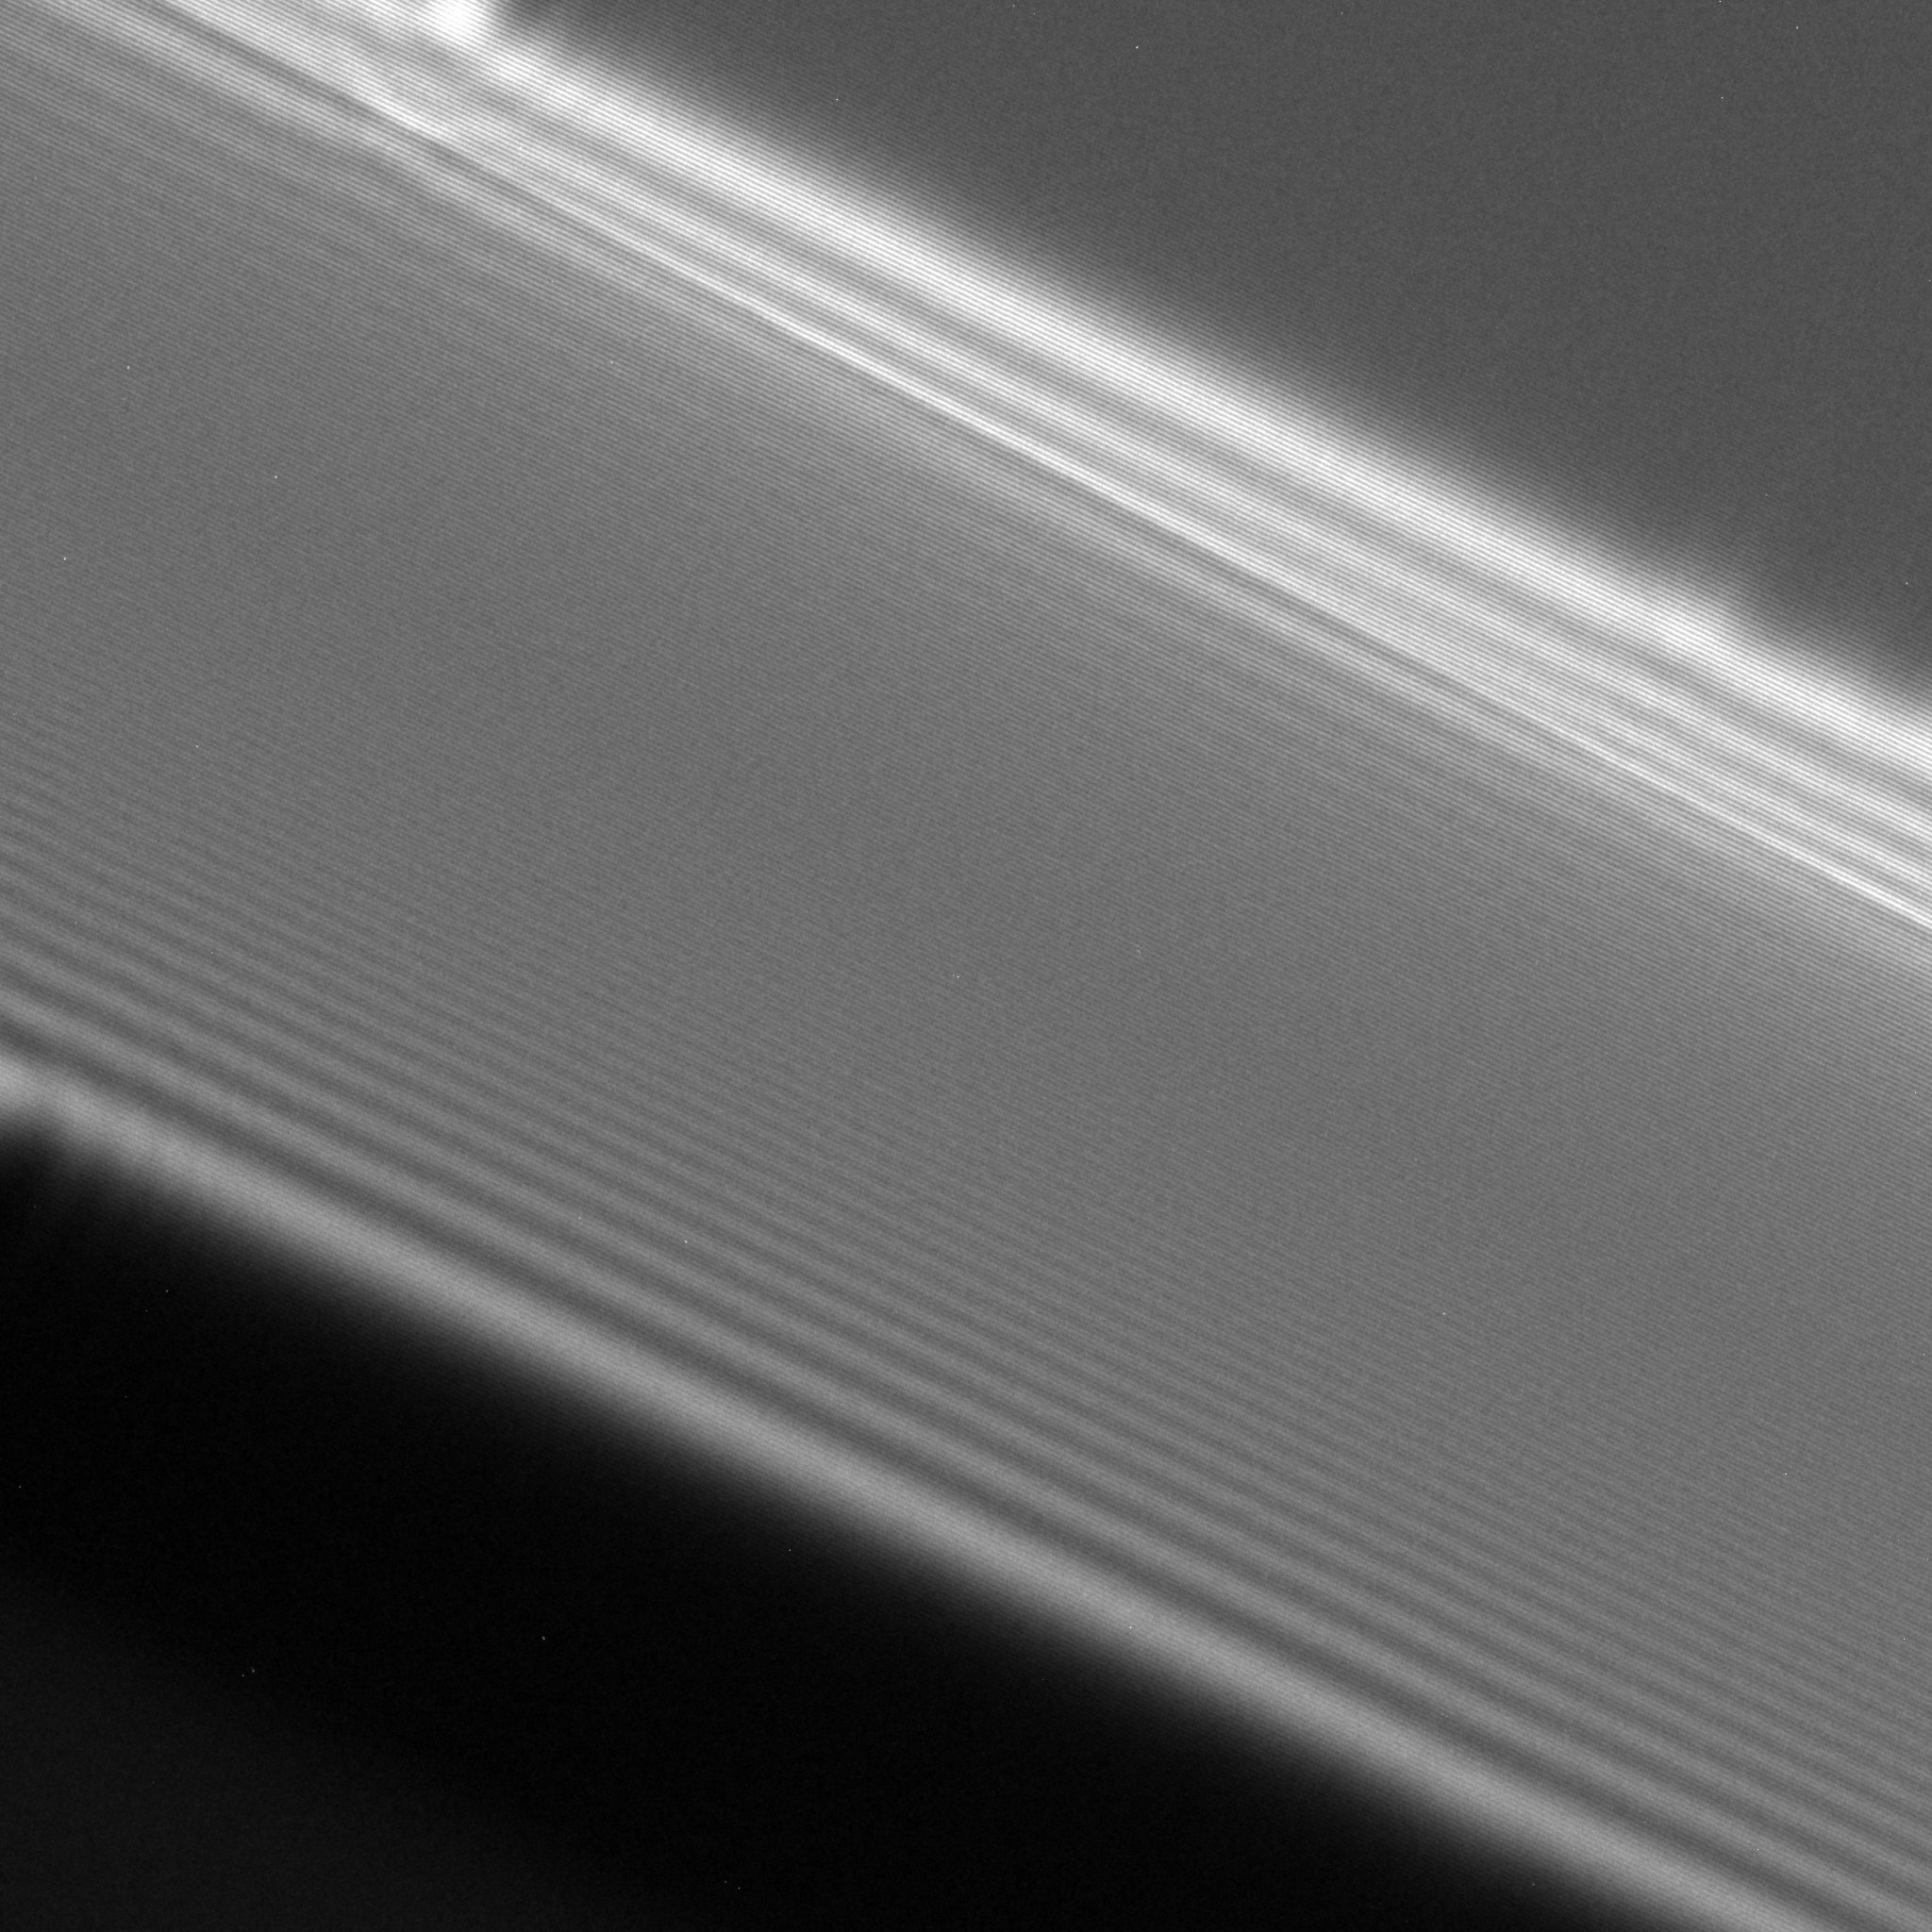
\includegraphics[width=\textwidth]{Gerüst/Abbildungen/Holographie/Probe/2_Probenhologramm_70.4V_Ltz_15500x.jpg}
         \caption{Objekthologramm}
         \label{P-NObjektEllip}
     \end{subfigure}
        \caption{Hologramm Aufnahme von Silikat Chip mit P-N Übergang mit Elliptischer Beleichtung}
        \label{P-NHologrammEllip}
\end{figure}

\begin{figure}
     \centering
     \begin{subfigure}[b]{0.3\textwidth}
         \centering
         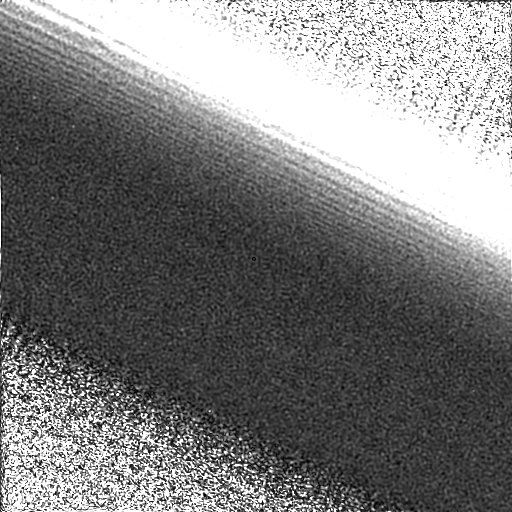
\includegraphics[width=\textwidth]{Holographie/Probe/3_Probenhologramm_70.4V_Ltz_15500x_iw_Amplitude.jpg}
         \caption{Amplitudenbild}
         \label{P-NAmpEllip}
     \end{subfigure}
     \hfill
     \begin{subfigure}[b]{0.3\textwidth}
         \centering
         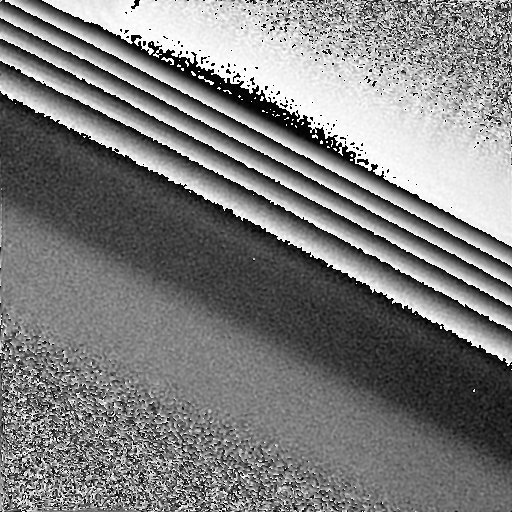
\includegraphics[width=\textwidth]{Holographie/Probe/5_Probenhologramm_70.4V_Ltz_15500x_iw_Phase_Wedge.jpg}
         \caption{Phasenbild, Wrapped}
         \label{P-NPhaseWEllip}
     \end{subfigure}
     \hfill
     \begin{subfigure}[b]{0.3\textwidth}
         \centering
         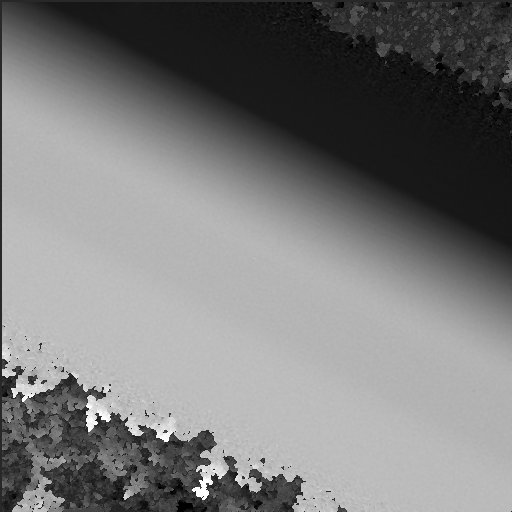
\includegraphics[width=\textwidth]{Holographie/Probe/6_Probenhologramm_70.4V_Ltz_15500x_iw_Phase_Wedge (unwrapped).jpg}
         \caption{Phasenbild, Unwrapped}
         \label{P-NphaseUEllip}
     \end{subfigure}
        \caption{}
        \label{AmpPhaseBildEllip}
\end{figure}